%% This template can be used to write a paper for
%% Computer Physics Communications using LaTeX.
%% For authors who want to write a computer program description,
%% an example Program Summary is included that only has to be
%% completed and which will give the correct layout in the
%% preprint and the journal.
%% The `elsarticle' style is used and more information on this style
%% can be found at 
%% http://www.elsevier.com/wps/find/authorsview.authors/elsarticle.
%%
%%
\documentclass[preprint,12pt]{elsarticle}

%% Use the option review to obtain double line spacing
%% \documentclass[preprint,review,12pt]{elsarticle}

%% Use the options 1p,twocolumn; 3p; 3p,twocolumn; 5p; or 5p,twocolumn
%% for a journal layout:
%% \documentclass[final,1p,times]{elsarticle}
%% \documentclass[final,1p,times,twocolumn]{elsarticle}
%% \documentclass[final,3p,times]{elsarticle}
%% \documentclass[final,3p,times,twocolumn]{elsarticle}
%% \documentclass[final,5p,times]{elsarticle}
%% \documentclass[final,5p,times,twocolumn]{elsarticle}

%% if you use PostScript figures in your article
%% use the graphics package for simple commands
%% \usepackage{graphics}
%% or use the graphicx package for more complicated commands
\usepackage{graphicx}
%% or use the epsfig package if you prefer to use the old commands
%% \usepackage{epsfig}

%% The amssymb package provides various useful mathematical symbols
\usepackage{amssymb}
%% The amsthm package provides extended theorem environments
%% \usepackage{amsthm}

%% Additional needed packages.
\usepackage{amsmath}
\usepackage{verbatim}
\usepackage{color}

%% The lineno packages adds line numbers. Start line numbering with
%% \begin{linenumbers}, end it with \end{linenumbers}. Or switch it on
%% for the whole article with \linenumbers after \end{frontmatter}.
\usepackage{lineno}
\usepackage{hyperref}

%% natbib.sty is loaded by default. However, natbib options can be
%% provided with \biboptions{...} command. Following options are
%% valid:

%%   round  -  round parentheses are used (default)
%%   square -  square brackets are used   [option]
%%   curly  -  curly braces are used      {option}
%%   angle  -  angle brackets are used    <option>
%%   semicolon  -  multiple citations separated by semi-colon
%%   colon  - same as semicolon, an earlier confusion
%%   comma  -  separated by comma
%%   numbers-  selects numerical citations
%%   super  -  numerical citations as superscripts
%%   sort   -  sorts multiple citations according to order in ref. list
%%   sort&compress   -  like sort, but also compresses numerical citations
%%   compress - compresses without sorting
%%
%% \biboptions{comma,round}

% \biboptions{}

\newcommand{\pdv}[2]{\frac{\partial{#1}}{\partial{#2}}}
\newcommand{\fp}[2]{\pdv{#1}{#2}}
\newcommand{\pdwc}[3]{\left(\fp{#1}{#2}\right)_{#3}}
%\newcommand{\ppdv}[3]{\displaystyle \frac{\partial^2 #1}{\partial #2\partial #3}}
\newcommand{\ppdv}[3]{\frac{\partial^2 #1}{\partial #2\partial #3}}
\newcommand{\oover}[1]{\ensuremath{\frac{1}{#1}}}

\newcommand{\vect}[1]{\boldsymbol{#1}}
\newcommand{\matr}[1]{\mathbf{#1}}
\newcommand{\dI}{\text{d}}
\newcommand{\odv}[2]{\frac{\dI #1}{\dI #2}}
\newcommand{\ddv}[2]{\odv{#1}{#2}}
\newcommand{\christ}[3]{\genfrac{\{}{\}}{0pt}{}{#1}{#2 #3}}
%\newcommand{\christ}[3]{\Gamma^{#1}_{#2 #3}}
%\newcommand{\ddv}[2]{\frac{\Delta #1}{\Delta #2}}
\newcommand{\collpdv}[2]{\pdv{#1}{#2}\Big|_{coll}}
\newcommand{\mfp}{\lambda}
\newcommand{\tmfp}{\tilde{\lambda}}
\newcommand{\mfpe}{\lambda_e}
\newcommand{\mfpei}{\lambda_{ei}}
\newcommand{\Zbar}{\bar{Z}}
\newcommand{\nue}{\nu_{e}}
\newcommand{\nuei}{\nu_{ei}}
\newcommand{\nutot}{\nu_{t}}
\newcommand{\vmag}{v}
\newcommand{\vth}{v_{th}}
\newcommand{\vn}{\vect{n}}
\newcommand{\E}{\vect{E}}
\newcommand{\B}{\vect{B}}
\newcommand{\tE}{\vect{\tilde{E}}}
\newcommand{\tEz}{\tilde{E}_z}
\newcommand{\tB}{\vect{\tilde{B}}}
\newcommand{\qe}{q_e}
\newcommand{\me}{m_e}
\newcommand{\kB}{k_B}
\newcommand{\crs}{\sigma}
\newcommand{\fM}{f_M}
\newcommand{\tfM}{\tilde{f}_M}
\newcommand{\tvfM}{\vect{\tilde{f}_M}}
\newcommand{\daf}{\delta f}
\newcommand{\fzero}{f_0}
\newcommand{\dafzero}{\delta f_0}
\newcommand{\vfzero}{\vect{f_0}}
\newcommand{\davfzero}{\vect{\delta f_0}}
\newcommand{\fone}{\vect{f_1}}
\newcommand{\fonez}{f_{1_z}}
\newcommand{\SM}{\vect{S}_M}
\newcommand{\MI}{\matr{I}}
\newcommand{\MA}{\matr{A}}
\newcommand{\intO}{\int_{\Omega}}
\newcommand{\intv}{\int_{\vmag}}
\newcommand{\IM}{\boldsymbol{\mathcal{M}}}
\newcommand{\ID}{\boldsymbol{\mathcal{D}}}
\newcommand{\IV}{\boldsymbol{\mathcal{V}}}
\newcommand{\IB}{\boldsymbol{\mathcal{B}}}
\newcommand{\anisomega}{\fone/\fzero}
\newcommand{\acl}{\vect{M}_{\left(\anisomega\right)}}

\newcommand{\Wzero}{\psi}
\newcommand{\Wone}{\matr{w}}
\newcommand{\Wcurl}{\vect{W_c}}
\newcommand{\Wdiv}{\vect{W_d}}



\newcommand{\figref}[1]{FIG.~\ref{#1}}
\newcommand{\refeq}[1]{\eqref{#1}}
\newcommand{\secref}[1]{Sec.~\ref{#1}}
\newcommand{\figscale}{0.5}

%% This list environment is used for the references in the
%% Program Summary
%%
\newcounter{bla}
\newenvironment{refnummer}{%
\list{[\arabic{bla}]}%
{\usecounter{bla}%
 \setlength{\itemindent}{0pt}%
 \setlength{\topsep}{0pt}%
 \setlength{\itemsep}{0pt}%
 \setlength{\labelsep}{2pt}%
 \setlength{\listparindent}{0pt}%
 \settowidth{\labelwidth}{[9]}%
 \setlength{\leftmargin}{\labelwidth}%
 \addtolength{\leftmargin}{\labelsep}%
 \setlength{\rightmargin}{0pt}}}
 {\endlist}

\journal{Computer Physics Communications}

\begin{document}

\begin{frontmatter}

%% Title, authors and addresses

%% use the tnoteref command within \title for footnotes;
%% use the tnotetext command for the associated footnote;
%% use the fnref command within \author or \address for footnotes;
%% use the fntext command for the associated footnote;
%% use the corref command within \author for corresponding author footnotes;
%% use the cortext command for the associated footnote;
%% use the ead command for the email address,
%% and the form \ead[url] for the home page:
%%
%% \title{Title\tnoteref{label1}}
%% \tnotetext[label1]{}
%% \author{Name\corref{cor1}\fnref{label2}}
%% \ead{email address}
%% \ead[url]{home page}
%% \fntext[label2]{}
%% \cortext[cor1]{}
%% \address{Address\fnref{label3}}
%% \fntext[label3]{}

\title{An~efficient kinetic modeling in plasmas by using the~AWBS transport equation}

%% use optional labels to link authors explicitly to addresses:
%% \author[label1,label2]{<author name>}
%% \address[label1]{<address>}
%% \address[label2]{<address>}

%\author[a]{M. Holec\corref{author}}
\author[a,b]{Authors}
%\author[b]{Third Author}

\cortext[author] {Corresponding author.\\\textit{E-mail address:} milan.holec@u-bordeaux.fr}
\address[a]{Centre Lasers Intenses et Applications, Universite de Bordeaux-CNRS-CEA, UMR 5107, F-33405 Talence, France}
%\address[b]{Second Address}

\begin{abstract}
The~AWBS Boltzmann transport equation for electrons equipped with 
a~simplified e-e collision operator~\cite{AWBS_PRL1986}
provides an~efficient, yet physically 
relevant, kinetic extension compared the~classical 
Spitzer-Harm heat flux (SH)
based on local approximation and flux-limiting.
This classical approach is widely used in plasma
kinetics models coupled to hydrodynamics. 
Even though SH reflects the~electron-electron collision effect, 
the essential physical properties
%, e.g. non-locality due to appropriate electron 
%distribution function, 
of the~electron transport cannot be modeled with 
an~explicitly local model. A~simple form of the~AWBS model opens a~way 
to couple kinetics to hydrodynamic codes while describing the~important 
physics correctly. Since the~electron-electron collision effect becomes 
especially important in the~case of low ion potential, we focus on presenting 
results related to low Z plasmas.
\end{abstract}

\begin{keyword}
%% keywords here, in the form: keyword \sep keyword
kinetics; hydrodynamics; nonlocal electron transport; laser-heated plasmas.

\end{keyword}

\end{frontmatter}

%%
%% Start line numbering here if you want
%%
 \linenumbers
\pagebreak
\tableofcontents
\pagebreak
%% main text
%\section{}
%\label{}
%---------------------------------------------------------------------
%---------------------------------------------------------------------

\section{Introduction}
\label{sec:Intro}

\section{The~AWBS nonlocal transport model}
\label{sec:AWBSmodel}
\begin{equation}
  \pdv{\ft}{t} + \vv\cdot\gx \ft + \tE \cdot\gv \ft =
  \vmag \frac{\nue}{2}\pdv{}{\vmag}\left(\ft - \fM\right) 
  + \frac{\nuei + \frac{\nue}{2}}{2} \frac{\partial^2 \ft}{\partial \vn^2}
  %\left(\pdv{}{\mu}\left((1 - \mu^2)\pdv{f}{\mu}\right)
  %+ \frac{1}{\sin^2(\phi)}\frac{\partial^2f}{\partial\theta^2} \right)  
  , \label{eq:AWBS_model}
\end{equation}
\cite{Fish_RMP1987}

\section{BGK, AWBS, and Fokker-Planck models in diffusive regime}
\label{sec:DiffusiveKinetics}

We can try to find an~approximate solution while using the~first term of
expansion in $\mfpe$ and $mu$as
\begin{equation}
  \tilde{f}(z, \vmag, \mu) = f^0(z, \vmag) + f^1(z, \vmag) \mfpei\mu .
  \label{eq:f_approximation}
\end{equation}


\subsection{The~BGK diffusive electron transport}
\label{sec:BGKDiffusiveRegime}

\begin{multline}
  \vn\cdot\nabla f + \frac{1}{\vmag} \left[ \tE\cdot\vn \pdv{f}{\vmag} 
  + \frac{\tE\cdot\vect{e}_\phi 
  - \vmag\tB\cdot\vect{e}_\theta}{\vmag}\pdv{f}{\phi}
  + \frac{\tE\cdot\vect{e}_\theta + \vmag\tB\cdot\vect{e}_\phi}
  {\vmag\sin(\phi)}\pdv{f}{\theta} \right] 
  =\\
  \frac{\left(\fM - f\right)}{\lambda^e} 
  + \frac{1}{2 \lambda^{ei}} 
  \left(\pdv{}{\mu}\left((1 - \mu^2)\pdv{f}{\mu}\right)
  + \frac{1}{\sin^2(\phi)}\frac{\partial^2f}{\partial\theta^2} \right) ,
  \label{eq:BGK_spherical}
\end{multline}
where $\mu = \cos(\phi)$, $\mfpe$ is the~electron-electron mean free path, and
$\mfpei$ is the~electron-ion mean free path. We also approximate
$\mfpe = \Zbar \mfpei$.

%We can try to find an~approximate solution while using the~first term of
%expansion in $\mfp$, $\cos(\phi)$, $\sin(\phi)$, $\sin(\theta)$, and $\fM$ as
%\begin{equation}
%  f = f^0 + f^1 \mfp\fM\cos(\phi) + f^2 \mfp\fM\sin(\phi)\sin(\theta),
%  \label{eq:f_approximation}
%\end{equation}
Clearly, $\pdv{\tilde{f}}{\theta} = 0$, and if $\tB = \tilde{B}_z\vect{e}_z$, 
there is no effect of magnetic field. We also assume, that 
$\nabla f = \pdv{f}{z}\vect{e}_z$ and appropriately 
$\tE = \tilde{E}_z\vect{e}_z$.
From the~orientation of the~Cartesian basis vectors and spherical 
basis vectors, one can find $\tE\cdot\vn = \tilde{E}_z \cos(\phi) = \mu$ and
$\tE\cdot\vect{e}_\phi = -\tilde{E}_z\sin(\phi)$. As a~result, the~analyzed
BGK equation reads
\begin{multline}
  \mu\pdv{}{z}\left( f^0 + f^1 \mfpei\mu \right) 
  + \frac{1}{\vmag} \left[ \tilde{E}_z\mu \pdv{}{\vmag} 
  \left( f^0 + f^1 \mfpei\mu \right) 
  - \frac{\tilde{E}_z\sin(\phi)}{\vmag}\pdv{}{\phi} 
  \left( f^0 + f^1 \mfpei\mu \right)
  \right] 
  =\\
  \frac{\left(\fM - \left( f^0 + f^1 \mfpei\mu \right) \right)}{\mfpe} 
  + \frac{1}{2 \mfpei}\pdv{}{\mu}\left((1 - \mu^2)
  \pdv{}{\mu}\left( f^0 + f^1 \mfpei\mu \right) \right) ,
  \label{eq:BGK_spherical}
\end{multline}

\begin{multline}
  \mu\pdv{f^0}{z} + \mu^2 \pdv{}{z}\left(f^1 \mfpei \right)
  + \frac{\tilde{E}_z}{\vmag} \left[ \mu \pdv{f^0}{\vmag} 
  + \mu^2 \pdv{}{\vmag} \left( f^1 \mfpei \right) 
  + \frac{1 - \mu^2}{\vmag}f^1 \mfpei
  \right] 
  =\\
  \frac{\fM - f^0}{\Zbar\mfpei} - \mu \frac{1}{\Zbar}f^1
  - \mu f^1 ,
  \label{eq:BGK_spherical}
\end{multline}
consequently, we have the~following anisotropy expansion 
$\mu^0, \mu^1, \mu^2, ...$ equations
\begin{eqnarray}
  \frac{\fM - f^0}{\Zbar\mfpei} &=& \frac{\tEz}{\vmag^2}f^1 \mfpei , 
  \nonumber \\
  \pdv{f^0}{z} + \frac{\tilde{E}_z}{\vmag}\pdv{f^0}{\vmag} &=& 
  - \frac{1}{\Zbar}f^1 - f^1 , 
  \nonumber \\ 
  \pdv{}{z}\left(f^1 \mfpei \right) 
  + \frac{\tilde{E}_z}{\vmag} \left[\pdv{}{\vmag} \left( f^1 \mfpei \right)
  - \frac{1}{\vmag}f^1 \mfpei \right] &=& 0 , \nonumber
\end{eqnarray}
which lead to the~definitions
\begin{eqnarray}
  f^0 &=& \fM + \frac{1}{\vmag}f^1 \Zbar\mfpei^2 ,
  \label{eq:BGK_f0} \\
  f^1 &=& - \frac{\Zbar}{\Zbar+1}
  \left[ \pdv{f^0}{z} + \frac{\tilde{E}_z}{\vmag}\pdv{f^0}{\vmag} \right] 
  \nonumber \\
  &=& - \frac{\Zbar}{\Zbar+1}
  \left[\frac{1}{\rho}\pdv{\rho}{z} + 
  \left( \frac{\vmag^2}{2 \vth^2} - \frac{3}{2}\right)
  \frac{1}{T}\pdv{T}{z} - \frac{\tilde{E}_z}{\vth^2} \right]\fM 
  %\nonumber \\
  %&=& - \frac{\Zbar}{\Zbar+1}
  %\left( \frac{\vmag^2}{2 \vth^2} - \frac{3}{2} - \alpha\right)
  %\frac{1}{T}\pdv{T}{z}\fM ,
  \label{eq:BGK_f1}
\end{eqnarray}

In order to ensure the~plasma to be quasi-neutral, the~zero-current condition
\begin{equation}
  \vect{j} = \int_0^{\infty}\int_{4\pi} \qe \vmag \vn f 
  \, \dI\vn~\vmag^2~\dI\vmag 
  = \vect{0} ,
  \label{eq:zero_current}
\end{equation}
can be achieved by providing a~consistent electric field in 
\refeq{eq:f_approximation}, i.e.
\begin{equation}
  \tE = \frac{\vth^2~\int_{4\pi} \vn\otimes\vn\cdot \int_0^{\infty} \vmag  
  \fM \frac{\mfp}{\alpha}\left(\frac{\nabla\rho}{\rho} + 
  \left( \frac{\vmag^2}{2 \vth^2} - \frac{3}{2}\right) 
  \frac{\nabla T}{T}\right)
  \vmag^2\, \dI\vmag\, \dI\vn}
  {\int_{4\pi} \vn\otimes\vn\cdot \int_0^{\infty} \vmag  
  \fM \frac{\mfp}{\alpha}\vmag^2\, \dI\vmag\, \dI\vn} ,
\end{equation}
which may be further simplified as
\begin{equation}
  \tE = \frac{\int_0^{\infty} \fM
  \frac{1}{2}\frac{\nabla T}{T}\vmag^9\, \dI\vmag}
  {\int_0^{\infty} \fM \vmag^7\, \dI\vmag} + 
  \vth^2\left(\frac{\nabla\rho}{\rho} - \frac{3}{2}\frac{\nabla T}{T} \right)
  = \vth^2\left(\frac{\nabla\rho}{\rho} + \frac{5}{2}\frac{\nabla T}{T} 
  \right) ,
\end{equation}
where it is worth mentioning, that the~part 
$\fM + \frac{\vmag\mfp}{\alpha} \pdv{f_1}{\vmag}$ of the~distribution
does not contribute to the~current since it is isotropic.
One can write the~quasi-neutral distribution function explicitly 
distinguishing between original part (blue color) and E field correction
(red color) as
\begin{equation}
  f \approx \fM \left(1 - \frac{\mfp}{\alpha}\vn\cdot\left( 
  \textcolor{blue}{
  \frac{\vmag^2}{2 \vth^2} - \frac{3}{2}
  }
  \textcolor{red}{
  - \frac{5}{2}
  }
  \right) \frac{\nabla T}{T} \right) 
  + \frac{\vmag\mfp}{\alpha} \pdv{f_1}{\vmag} .
  \label{eq:f_localized_quasineutral}
\end{equation}
which leads to the~resulting heat flux
\begin{equation}
  \vect{q}_H = \int_{4\pi}\int_0^{\infty} \frac{\me \vmag^2}{2} \vmag \vn f 
  \vmag^2\, \dI\vmag\, \dI\vn = \frac{4\pi}{3}\frac{\me}{2}
  \frac{1}{\alpha \crs\rho}
  \int_0^{\infty} \left( 
  \textcolor{blue}{
  \frac{\vmag^2}{2 \vth^2} - \frac{3}{2}
  }
  \textcolor{red}{
  - \frac{5}{2}
  }
  \right) \vmag^9 \fM\, \dI\vmag \frac{\nabla T}{T} .
  \nonumber
\end{equation} 
Based on the~Gauss integral formula
\begin{equation}
  \int \vmag^{2s+1} \exp\left(-\frac{\vmag^2}{2\vth^2}\right)\, \dI\vmag = 
  \frac{s!~(2 \vth^2)^{s+1}}{2}
  \nonumber 
\end{equation}
and Maxwell-Boltzmann distribution \refeq{eq:MBdistribution} the~heat flux can 
be written as
\begin{equation}
  \vect{q}_H = \frac{4\pi}{3}\frac{\me}{2}\frac{1}{\alpha \crs\rho}
  \frac{\rho}{\vth^3 \left( 2 \pi \right)^{3/2}}
  \frac{4!~2^4 \vth^{10}}{T} \left( 
  \textcolor{blue}{
  5 - \frac{3}{2}
  }
  \textcolor{red}{
  - \frac{5}{2}
  }
  \right) \nabla T 
  = \frac{\me}{\alpha \crs}\frac{128}{\sqrt{2 \pi}}
  \left(\frac{\kB}{\me}\right)^{\frac{7}{2}}T^{\frac{5}{2}} \nabla T .
  \label{eq:Lorentz_flux}
\end{equation} 
In conclusion, equation \refeq{eq:Lorentz_flux} provides nothing else than
the~well known Lorentz approximation heat flux and its nonlinearity $2.5$
in temperature. What is worth mentioning is the~effect of E field 
(quasi-neutrality), which reduces the~flux of about	71.4$\%$ 
(also assuming constant density).


Finally, one can find the~approximate solution
\begin{equation}
  \tilde{f} = \fM - \mfpei\frac{\Zbar}{\Zbar+1}
  \left( \frac{\vmag^2}{2 \vth^2} - \frac{3}{2} - \alpha\right)
  \frac{\vn\cdot\nabla T}{T}\fM .
  \label{eq:BGK_approximate_solution}
\end{equation}


\subsection{The~AWBS diffusive electron transport}
\label{sec:AWBSDiffusiveRegime}

The~AWBS electron transport equation in 6D reads
\begin{multline}
  \vn\cdot\nabla f + \frac{1}{\vmag} \left[ \tE\cdot\vn \pdv{f}{\vmag} 
  + \frac{\tE\cdot\vect{e}_\phi 
  - \vmag\tB\cdot\vect{e}_\theta}{\vmag}\pdv{f}{\phi}
  + \frac{\tE\cdot\vect{e}_\theta + \vmag\tB\cdot\vect{e}_\phi}
  {\vmag\sin(\phi)}\pdv{f}{\theta} \right] 
  =\\
  \frac{\vmag}{\lambda^e}\pdv{}{\vmag}\left(f - f_M\right) 
  + \left(\frac{1}{\mfpei} + \frac{1}{\mfpe} \right) \frac{1}{2}
  \left(\pdv{}{\mu}\left((1 - \mu^2)\pdv{f}{\mu}\right)
  + \frac{1}{\sin^2(\phi)}\frac{\partial^2f}{\partial\theta^2} \right) ,
  \label{eq:AWBS_spherical}
\end{multline}
where $\mu = \cos(\phi)$, $\mfpe$ is the~electron-electron mean free path, and
$\mfpei$ is the~electron-ion mean free path, and $\mfpe = \Zbar \mfpei$.

We can try to find an~approximate solution while using the~first term of
expansion in $\mfpe$ and $\mu$ as
\begin{equation}
  \tilde{f}(z, \vmag, \mu) = f^0(z, \vmag) + f^1(z, \vmag) \mfpei\mu .
  \label{eq:f_approximation}
\end{equation}
Clearly, $\pdv{\tilde{f}}{\theta} = 0$, and if $\tB = \tilde{B}_z\vect{e}_z$, 
there is no effect of magnetic field. We also assume, that 
$\nabla f = \pdv{f}{z}\vect{e}_z$ and appropriately 
$\tE = \tilde{E}_z\vect{e}_z$.
From the~orientation of the~Cartesian basis vectors and spherical 
basis vectors, one can find $\tE\cdot\vn = \tilde{E}_z \cos(\phi) = \mu$ and
$\tE\cdot\vect{e}_\phi = -\tilde{E}_z\sin(\phi)$. As a~result, the~analyzed
AWBS equation reads
\begin{multline}
  \mu\pdv{}{z}\left( f^0 + f^1 \mfpei\mu \right) 
  + \frac{1}{\vmag} \left[ \tilde{E}_z\mu \pdv{}{\vmag} 
  \left( f^0 + f^1 \mfpei\mu \right) 
  - \frac{\tilde{E}_z\sin(\phi)}{\vmag}\pdv{}{\phi} 
  \left( f^0 + f^1 \mfpei\mu \right)
  \right] 
  =\\
  \frac{\vmag}{\mfpe}\pdv{}{\vmag}
  \left(\left( f^0 + f^1 \mfpei\mu \right) -\fM\right)
  + \frac{\Zbar +1}{2 \mfpei \Zbar}\pdv{}{\mu}\left((1 - \mu^2)
  \pdv{}{\mu}\left( f^0 + f^1 \mfpei\mu \right) \right) ,
  \label{eq:AWBS_spherical}
\end{multline}

\begin{multline}
  \mu\pdv{f^0}{z} + \mu^2 \pdv{}{z}\left(f^1 \mfpei \right)
  + \frac{\tilde{E}_z}{\vmag} \left[ \mu \pdv{f^0}{\vmag} 
  + \mu^2 \pdv{}{\vmag} \left( f^1 \mfpei \right) 
  + \frac{1 - \mu^2}{\vmag}f^1 \mfpei
  \right] 
  =\\
  \frac{\vmag}{\Zbar\mfpei}\pdv{}{\vmag}
  \left( f^0 -\fM\right)
  + \mu\frac{\vmag}{\Zbar\mfpei}\pdv{\left(f^1 \mfpei\right)}{\vmag} 
  - \mu \frac{\Zbar + 1}{\Zbar}f^1 ,
  \label{eq:AWBS_spherical}
\end{multline}
consequently, we have the~following anisotropy expansion 
$\mu^0, \mu^1, \mu^2, ...$ equations
\begin{eqnarray}
  \frac{\vmag}{\Zbar\mfpei}\pdv{}{\vmag}
  \left( f^0 -\fM\right) &=& \frac{\tEz}{\vmag^2}f^1 \mfpei , 
  \nonumber \\
  \pdv{f^0}{z} + \frac{\tilde{E}_z}{\vmag}\pdv{f^0}{\vmag} &=& 
  \frac{\vmag}{\Zbar\mfpei}\pdv{\left(f^1 \mfpei\right)}{\vmag}  
  - \frac{\Zbar + 1}{\Zbar} f^1 , 
  \nonumber \\ 
  \pdv{}{z}\left(f^1 \mfpei \right) 
  + \frac{\tilde{E}_z}{\vmag} \left[\pdv{}{\vmag} \left( f^1 \mfpei \right)
  - \frac{1}{\vmag}f^1 \mfpei \right] &=& 0 , \nonumber
\end{eqnarray}
which lead to the~definitions
\begin{eqnarray}
  \pdv{}{\vmag}\left( f^0 -\fM\right) &=& \frac{1}{\vmag^2}f^1 \Zbar\mfpei^2 ,
  \label{eq:AWBS_f0} \\
  \frac{\vmag}{\Zbar\mfpei}\pdv{\left(f^1 \mfpei\right)}{\vmag}  
  - \frac{\Zbar + 1}{\Zbar} f^1 &=&
  \pdv{f^0}{z} + \frac{\tilde{E}_z}{\vmag}\pdv{f^0}{\vmag}
  \nonumber \\  
  \frac{\vmag}{\Zbar}\pdv{f^1}{\vmag} + \frac{4}{\Zbar}f^1 
  - \frac{\Zbar + 1}{\Zbar} f^1 &=&
  \pdv{f^0}{z} + \frac{\tilde{E}_z}{\vmag}\pdv{f^0}{\vmag}
  \nonumber \\
  \pdv{f^1}{\vmag} + \frac{1}{\vmag}(3-\Zbar)f^1
  &=&
  \frac{\Zbar}{\vmag}\left(\frac{1}{\rho}\pdv{\rho}{z} + 
  \left( \frac{\vmag^2}{2 \vth^2} - \frac{3}{2}\right)
  \frac{1}{T}\pdv{T}{z} - \frac{\tilde{E}_z}{\vth^2}\right)\fM .
  \label{eq:AWBS_f1}
\end{eqnarray}


\subsection{The~Fokker-Planck diffusive electron transport}
\label{sec:FPDiffusiveRegime}
\begin{equation}
  \vtwoh = \sqrt{\frac{2 \kB T}{\me}} = 1 / j,
  \nonumber
\end{equation}
\begin{eqnarray}
  A &=& -\frac{\me^2 \vtwoh^2 \tE}{2 \pi e^4 n_e \lnc} = - \frac{m E}{2\pi j^2 e^3 n_e \lnc}
  , \nonumber \\
  B &=& \frac{\me^2 \vtwoh^4 |\nabla T|}{2 \pi e^4 n_e \lnc T} = \frac{2 \kB^2 T |\nabla T|}{\pi e^4 n_e \lnc}
  , \nonumber
\end{eqnarray}
\begin{equation}
  \frac{A}{B} = - \frac{|\tE| T}{\vtwoh^2 |\nabla T|} ,
  \nonumber
\end{equation}
\begin{equation}
  \tE = -\frac{3}{2}\frac{\vtwoh^2}{2}\frac{\gamma_T}{\gamma_E}
  \frac{\nabla T}{T} ,
  \nonumber
\end{equation}
From Eq. (24) CSR, we can write the~form of $f_1$ including both $\nabla T$ 
and $\tE$ effects as
\begin{equation}
  f_1(\vmag, \theta) = \cos(\theta) \frac{B}{\Zbar}\left( d_T(\vmag/\vtwoh) 
  + \frac{A}{B} d_E(\vmag/\vtwoh) \right) \fM(\vmag)  ,
  \nonumber
\end{equation}
where in the~case of vanishing current one gets
\begin{equation}
  \frac{A}{B} = \frac{3}{2}\frac{\gamma_T}{2 \gamma_E} ,
  \nonumber
\end{equation}
i.e.
\begin{equation}
  f_1(\vmag, \theta) = \cos(\theta) \frac{\me^2}{4 \pi e^4\lnc} 
  \frac{\vtwoh^4}{\Zbar}\left( 2 d_T(\vmag/\vtwoh) 
  + \frac{3}{2}\frac{\gamma_T}{\gamma_E} d_E(\vmag/\vtwoh) \right) 
  \frac{\fM(\vmag)}{n_e}\frac{\nabla T}{T}  ,
  \label{eq:f1_SH}
\end{equation}
where $d_T(x) = \Zbar D_{T}(x) / B$ and $d_E(x) = \Zbar D_{E}(x) / A$ 
are represented by numerical values in TABLE I and TABLE II in 
\cite{SH_PR1953}, respectively. 
In the~case of high $\Zbar$ limit, $\gamma_T \rightarrow 1$,
$\gamma_E \rightarrow 1$, $d_E(x) = x^4$, and $d_T(x) = x^4 (2.5 - x^2)/2$
\cite{SH_PR1953}, which leads to the~standard Lorentz gas model
\begin{equation}
   f_1(\vmag, \theta) = \cos(\theta) \frac{\me^2}{4 \pi e^4\lnc} 
  \frac{\vmag^4}{\Zbar}\left( 4 - \frac{\vmag^2}{\vtwoh^2} \right) 
  \frac{\fM(\vmag)}{n_e}\frac{\nabla T}{T}  ,
  \label{eq:f1_Lorentz} 
\end{equation}

\cite{Rosenbluth_PR1957}, \cite{Longmire_1963}, \cite{Shkarofsky_1966}

\subsection{Summary of BGK, AWBS, and Fokker-Planck diffusion}
\label{sec:SummaryDiffusiveKinetics}

\begin{figure}[tbh]
  \begin{center}
    \begin{tabular}{c}
      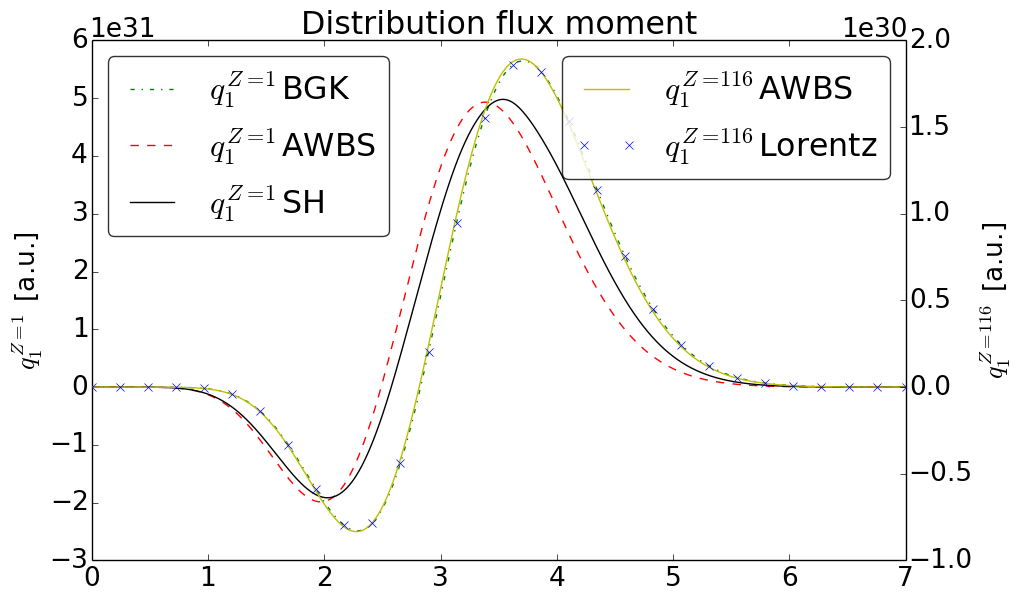
\includegraphics[width=0.8\textwidth]{q1s.png}
    \end{tabular}
  \caption{  
  The~flux velocity moment of the~anisotropic part of the~electron distribution 
  function in low $Z=1$ and high $Z=116$ plasmas in diffusive regime.}
  \end{center}
  \label{fig:q1s_summary}
\end{figure}

\begin{table}
\begin{center}
  \begin{tabular}{c|ccccc}
    \hline\hline\\
    %$\Zbar$ & $1$ & $2$ & $4$ & $16$ & $\infty$ \\\\
    & $\,\Zbar=1\,$ & $\,\Zbar=2\,$ & $\,\Zbar=4\,$ & $\,\Zbar=16\,$ & $\,\Zbar=116\,$ \\\\
    \hline\\
    $error(\vect{q}_{AWBS})$ & 0.057 & 0.004 & 0.038 & 0.049 & 0.004 \\\\
    \hline\hline
  \end{tabular}
  \caption{
  Relative $error(\vect{q}_{AWBS}) = |\vect{q}_{AWBS} - \vect{q}_{SH}| / \vect{q}_{SH}$ of the~AWBS
  kinetic model equation \refeq{eq:AWBS_model} showing the~discrepancy 
  (maximum around 5$\%$) with respect to the~original solution of 
  the~heat flux given by Spitzer and Harm \cite{SH_PR1953}.
  }
\end{center}
\end{table}

\section{Benchmarking the~AWBS nonlocal transport model}
\label{sec:BenchmarkingAWBS}

\subsection{Review of simulation codes}
\label{sec:ReviewOfCodes}

\subsubsection{C7}
\label{sec:C7code}
Since in the~laser heated plasmas the~Knudsen number 
Kn$ = \frac{\vth}{\nu_t(\vth) L} \in (0, 1)$, i.e. the~collisionality in 
the~kinetics of electrons plays always an~important effect for thermal-like 
particles, the~electron distribution 
function can be treated as out-of-equilibrium approximation 
\begin{equation}
  f = \fM + \daf ,
  \label{eq:OOE_outofeq}
\end{equation}  
where the~consequent AWBS model reads
\begin{multline}
  \vmag\vn\cdot\nabla (\fM + \daf) + \tE\cdot\vn \left(\pdv{\fM}{\vmag} 
  + \pdv{\daf}{\vmag}\right) 
  + \frac{\tE\cdot\vect{e}_\theta}{\vmag}\pdv{\daf}{\theta}
  = \\
  \vmag \frac{\nue}{2} \pdv{\daf}{\vmag} 
  + \left(\nuei + \frac{\nue}{2}\right) (\fzero - (\fM + \daf)) ,
  \label{eq:OOE_AWBS_model}
\end{multline}
or its 1D version
\begin{multline}
  \vmag\mu\pdv{}{z}(\fM + \daf) + \tEz\mu\left(\pdv{\fM}{\vmag} 
  + \pdv{\daf}{\vmag}\right) 
  + \frac{\tEz(1-\mu^2)}{\vmag}\pdv{\daf}{\mu}
  = \\
  \vmag \frac{\nue}{2} \pdv{\daf}{\vmag} 
  + \left(\nuei + \frac{\nue}{2}\right) (\fzero - (\fM + \daf)) ,
  \label{eq:OOE_AWBS_model_1D}
\end{multline}
where $\tE\cdot\vect{e}_\theta = \tEz\sin(\theta)$ and $\pdv{}{\theta} = \sin(\theta)\pdv{}{\mu}$, $\mu = \cos(\theta)$.
\begin{multline}
  \left(\vmag \frac{\nue}{2} - \tEz\mu\right) \pdv{\daf}{\vmag} = 
  \vmag\mu\pdv{\daf}{z} + \vmag\mu\pdv{\fM}{z} + \tEz\mu\pdv{\fM}{\vmag} \\ 
  + \frac{\tEz(1-\mu^2)}{\vmag}\pdv{\daf}{\mu}
  - \left(\nuei + \frac{\nue}{2}\right) (\fzero - (\fM + \daf))
  ,
  \nonumber
\end{multline}
we adopt $\daf(\vmag, \mu) = \dafzero(\vmag) + \mu\dafone(\vmag)$, 
which leads to
\begin{multline}
  \left(\vmag \frac{\nue}{2} - \tEz\mu\right) \pdv{}{\vmag}
  (\dafzero + \mu\dafone) = 
  \vmag\mu\pdv{}{z}(\dafzero + \mu\dafone) + \vmag\mu\pdv{\fM}{z} 
  + \tEz\mu\pdv{\fM}{\vmag} \\ 
  + \frac{\tEz(1-\mu^2)}{\vmag}\dafone
  + \left(\nuei + \frac{\nue}{2}\right) \mu\dafone
  ,
  \nonumber
\end{multline}
\begin{eqnarray}
  \vmag \frac{\nue}{2}\pdv{\dafzero}{\vmag}
  - \tEz\mu^2 \pdv{\dafone}{\vmag}
  &=& 
  \vmag\mu^2\pdv{\dafone}{z}
  + \frac{\tEz(1-\mu^2)}{\vmag}\dafone
  , \nonumber \\
  \mu\vmag \frac{\nue}{2}\pdv{\dafone}{\vmag} - \tEz\mu \pdv{\dafzero}{\vmag}
  &=& 
  \vmag\mu\pdv{\dafzero}{z}
  + \vmag\mu\pdv{\fM}{z} + \tEz\mu\pdv{\fM}{\vmag}  
  + \left(\nuei + \frac{\nue}{2}\right) \mu\dafone
  ,
  \nonumber
\end{eqnarray}


\subsubsection{ALADIN}
\label{sec:ALADINcode}

\subsubsection{IMPACT}
\label{sec:IMPACTcode}

\subsubsection{CALDER}
\label{sec:CALDERcode}

\subsection{Simulation results}
\label{sec:SimulationResults}

\begin{figure}[tbh]
  \begin{center}
    \begin{tabular}{cc}
      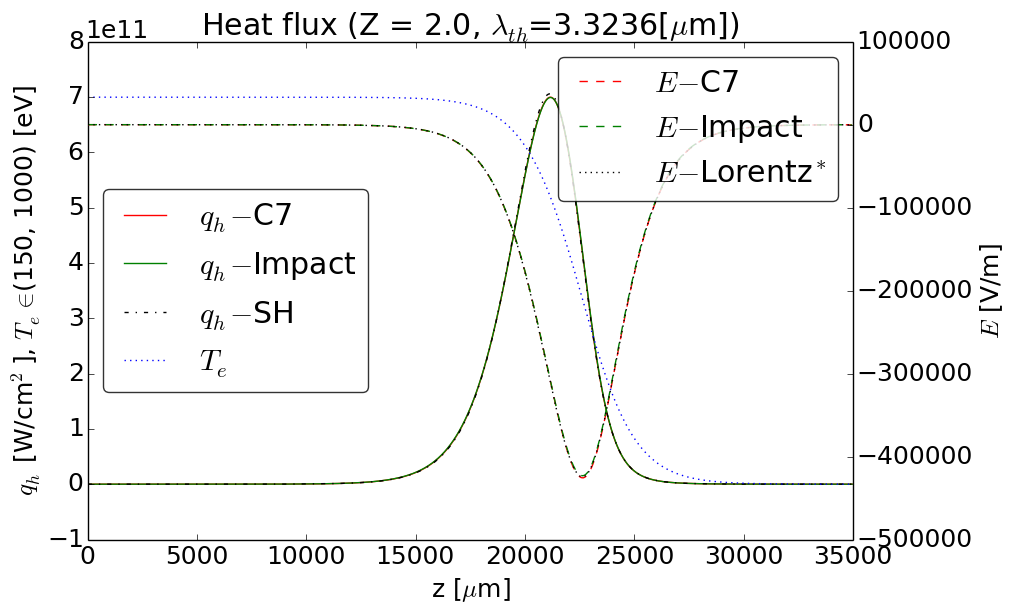
\includegraphics[width=\figscale\textwidth]{../VFPdata/C7_Impact_case1_heatflux.png} &
      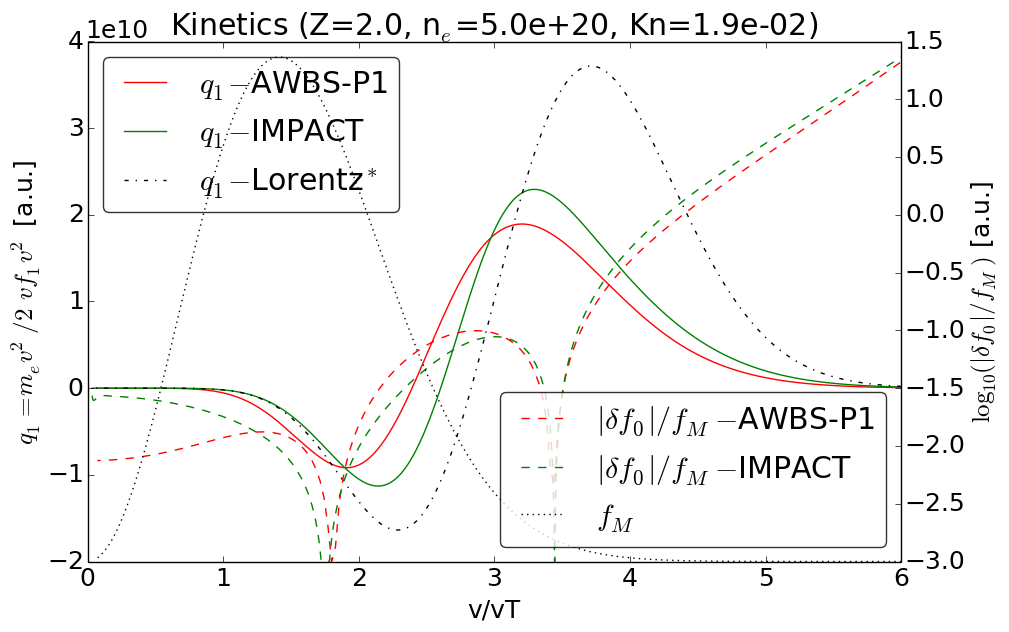
\includegraphics[width=\figscale\textwidth]{../VFPdata/C7_Impact_case1_kinetics.png}
    \end{tabular}
  \caption{  
  Snapshot 12 ps. Left: correct steady solution. Right: correct comparison to kinetic profiles at point 437 $\mu$m by IMPACT.}
  \end{center}
  \label{fig:C7_IMPACT_case1}
\end{figure}

\begin{figure}[tbh]
  \begin{center}
    \begin{tabular}{cc}
      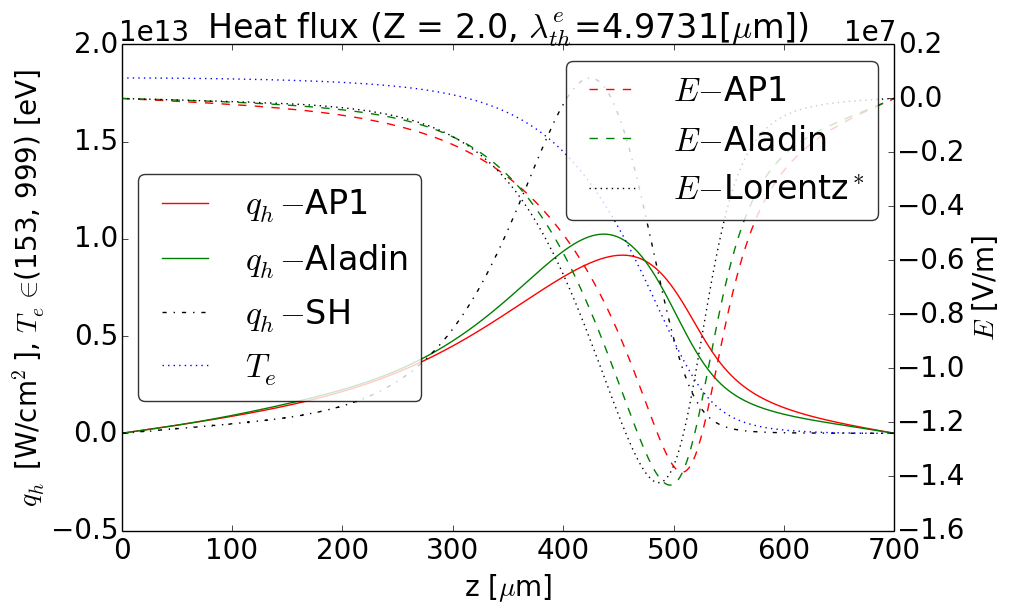
\includegraphics[width=\figscale\textwidth]{../VFPdata/C7_Aladin_case1_heatflux.png} &
      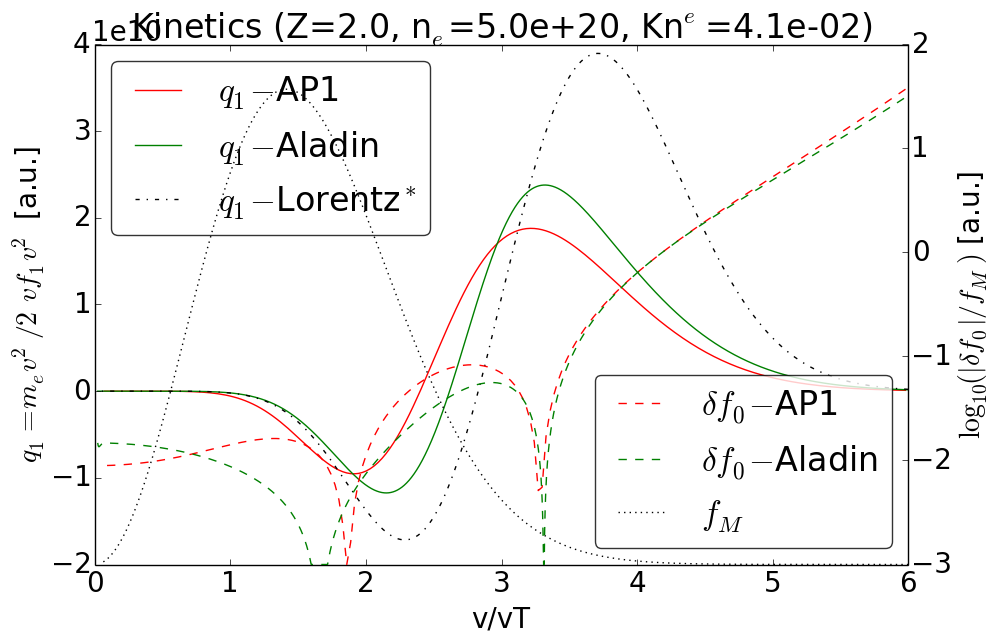
\includegraphics[width=\figscale\textwidth]{../VFPdata/C7_Aladin_case1_kinetics.png}
    \end{tabular}
  \caption{  
  Snapshot 12 ps. Left: correct steady solution. Right: correct comparison to kinetic profiles at point 442 $\mu$m by ALADIN.}
  \end{center}
  \label{fig:C7_ALADIN_case1}
\end{figure}

\begin{figure}[tbh]
  \begin{center}
    \begin{tabular}{cc}
      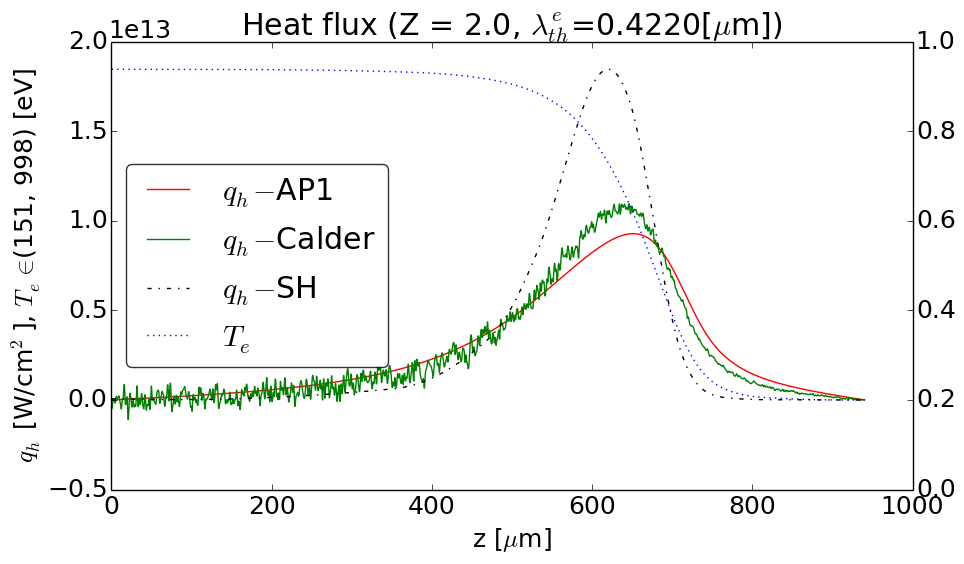
\includegraphics[width=\figscale\textwidth]{../VFPdata/C7_Calder_case1_heatflux.png} & 
      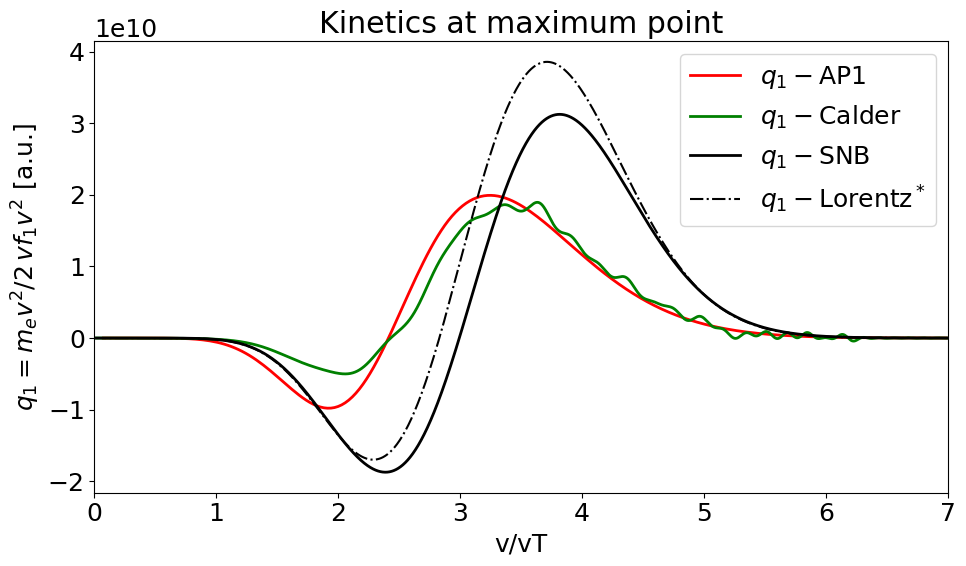
\includegraphics[width=\figscale\textwidth]{../VFPdata/C7_Calder_case1_kinetics.png}
    \end{tabular}
  \caption{  
  Snapshot 11 ps. Left: correct steady solution. Right: Kinetic profiles at point of maximum flux by C7. Kinetics profiles by CALDER to be added.
  }
  \end{center}
  \label{fig:C7_CALDER_case1}
\end{figure}

\begin{figure}[tbh]
  \begin{center}
    \begin{tabular}{cc}
      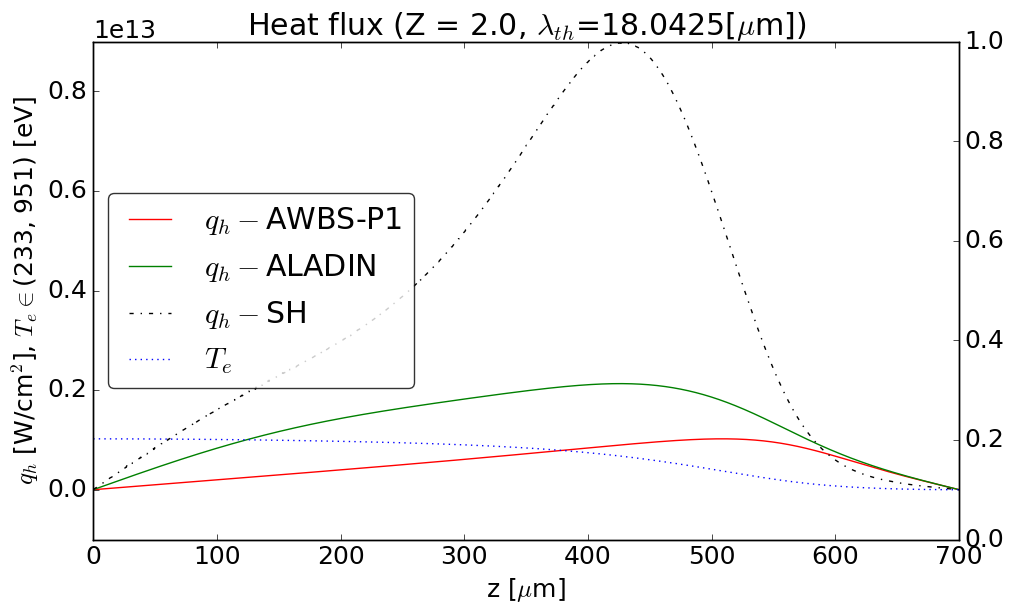
\includegraphics[width=\figscale\textwidth]{../VFPdata/C7_Aladin_case2_heatflux.png} &
      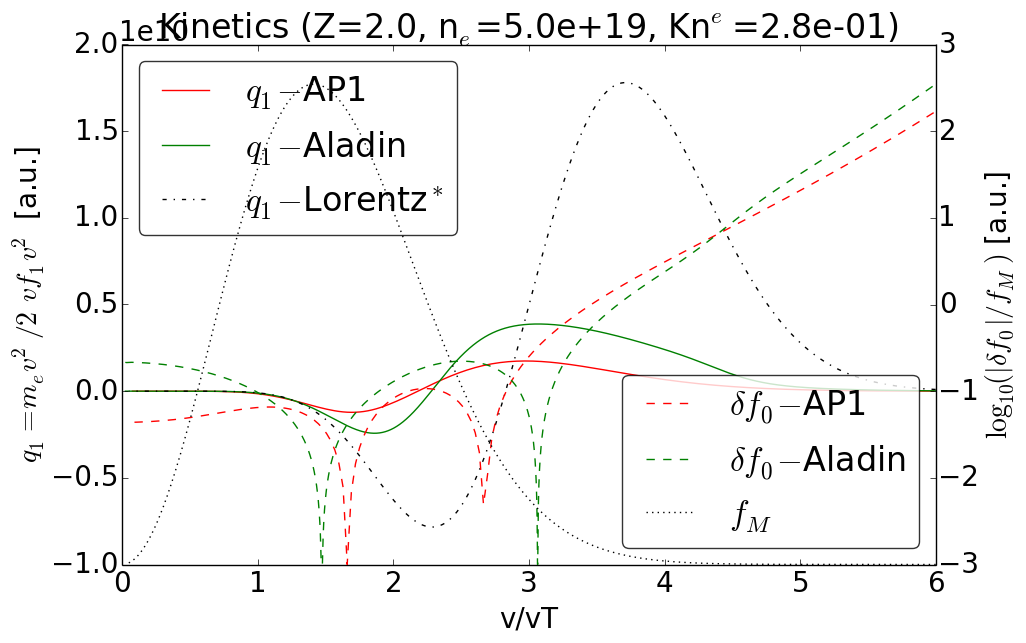
\includegraphics[width=\figscale\textwidth]{../VFPdata/C7_Aladin_case2_kinetics.png}
    \end{tabular}
  \caption{  
  Snapshot 12 ps. Left: correct steady solution. Right: correct comparison to kinetic profiles at point 480 $\mu$m  by ALADIN.
  }
  \end{center}
  \label{fig:C7_ALADIN_case2}
\end{figure}

\begin{figure}[tbh]
  \begin{center}
    \begin{tabular}{cc}
      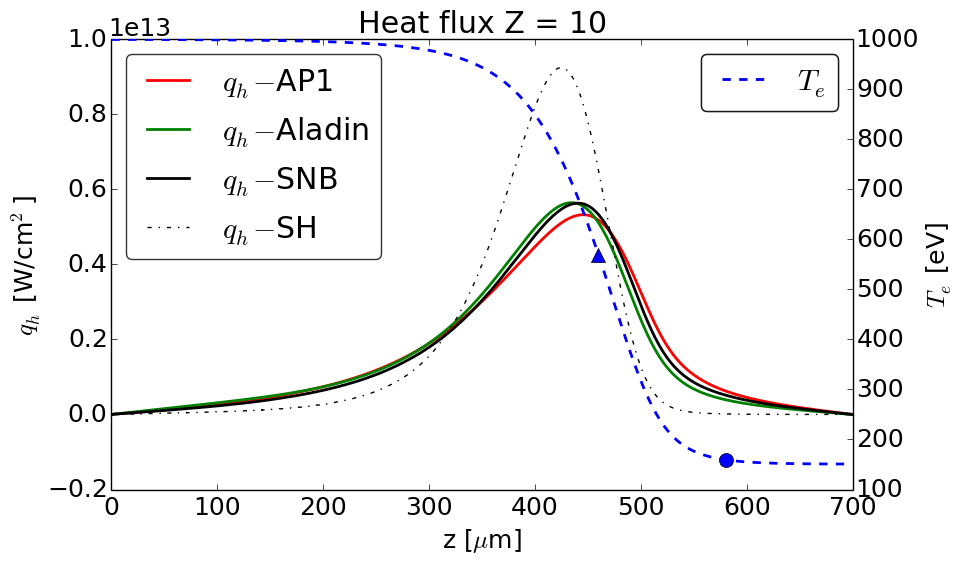
\includegraphics[width=\figscale\textwidth]{../VFPdata/C7_Aladin_case3_heatflux.png} &
      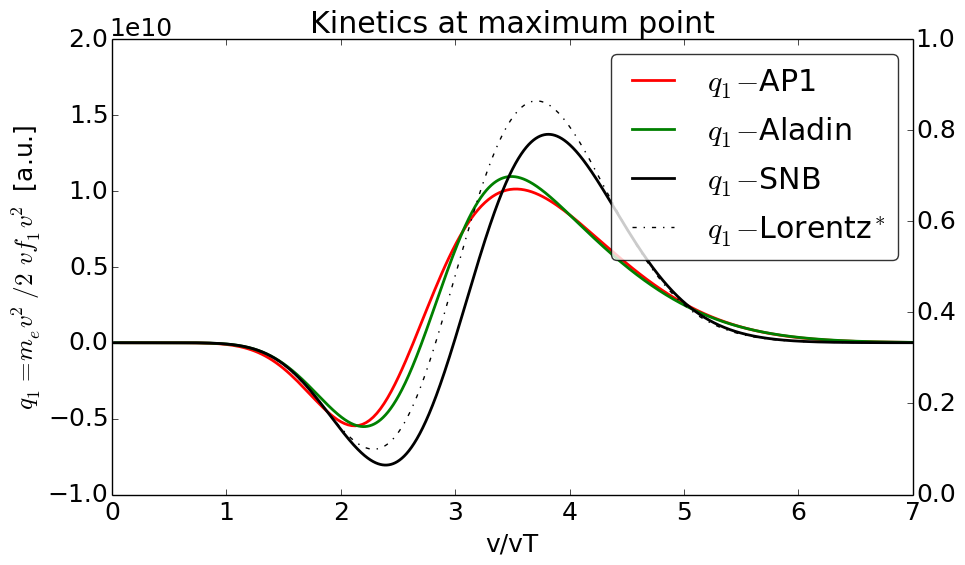
\includegraphics[width=\figscale\textwidth]{../VFPdata/C7_Aladin_case3_kinetics.png}
    \end{tabular}
  \caption{  
  Snapshot 12 ps. Left: correct steady solution. Right: correct comparison to kinetic profiles at point 442 $\mu$m by ALADIN.
  }
  \end{center}
  \label{fig:C7_ALADIN_case3}
\end{figure}

\begin{figure}[tbh]
  \begin{center}
    \begin{tabular}{cc}
      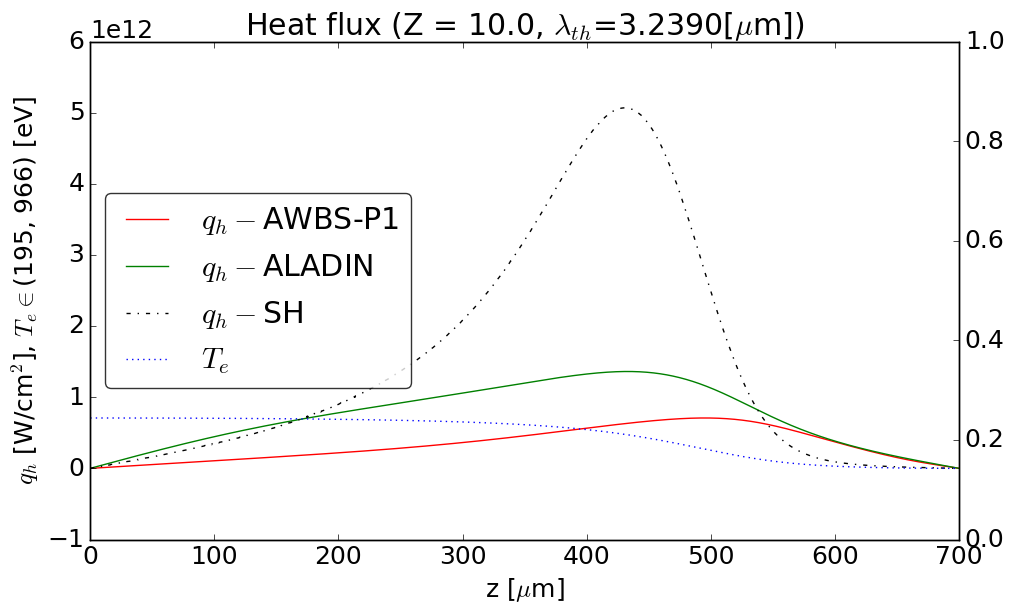
\includegraphics[width=\figscale\textwidth]{../VFPdata/C7_Aladin_case4_heatflux.png} & 
      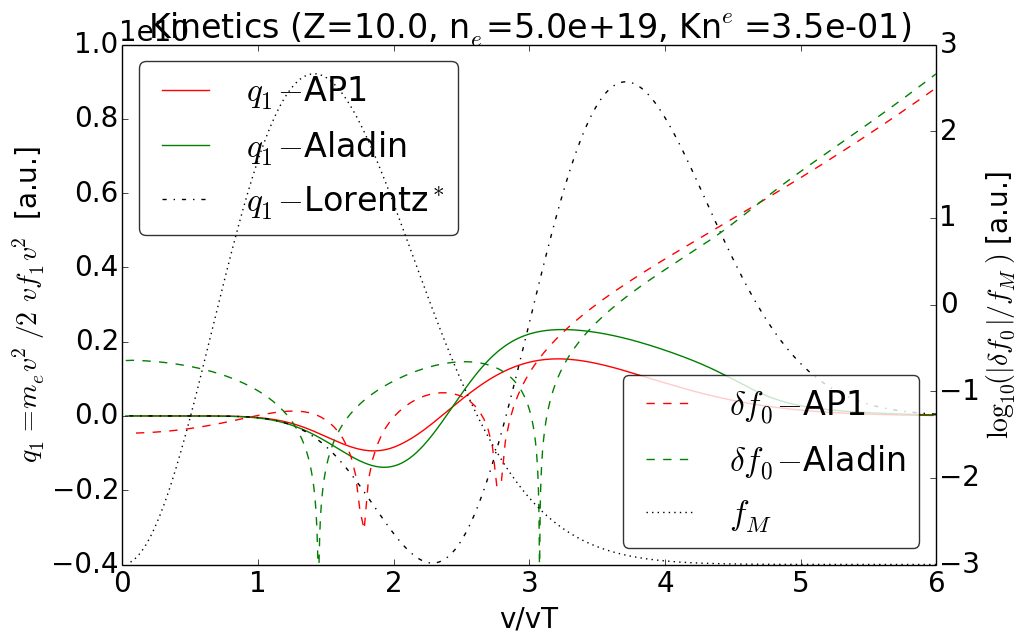
\includegraphics[width=\figscale\textwidth]{../VFPdata/C7_Aladin_case4_kinetics.png}
    \end{tabular}
  \caption{  
  Snapshot 12 ps. Left: correct steady solution. Right: correct comparison to kinetic profiles at point 480 $\mu$m by ALADIN.
  }
  \end{center}
  \label{fig:C7_ALADIN_case4}
\end{figure}

\clearpage

\begin{figure}[tbh]
  \begin{center}
    \begin{tabular}{c}
      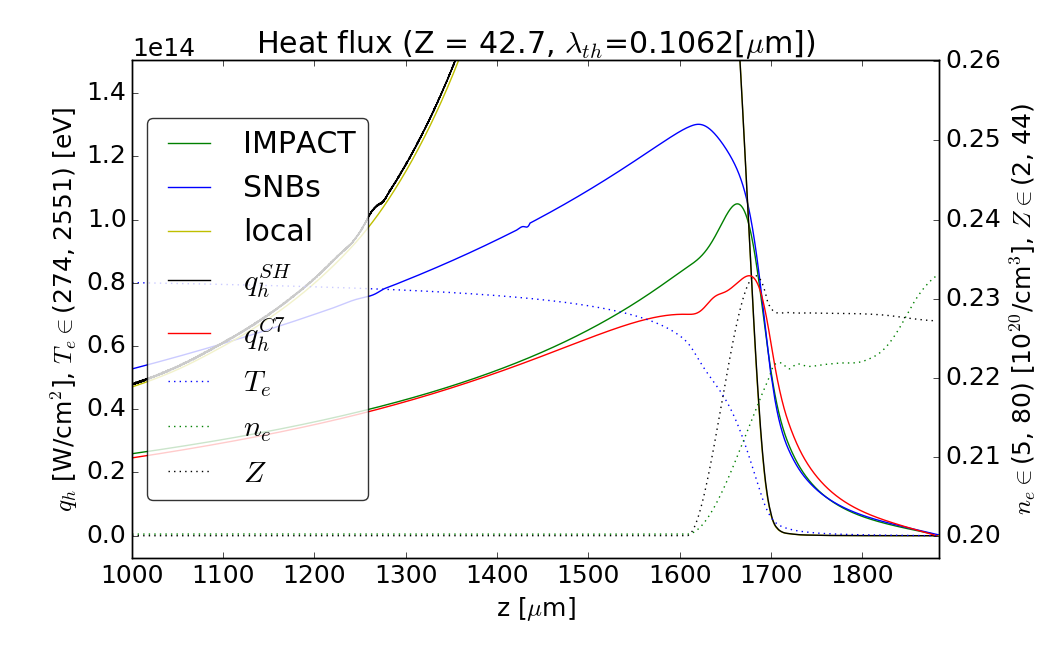
\includegraphics[width=1.0\textwidth]{../VFPdata/GD_Hohlraum/fluxes_10ps.png} 
    \end{tabular}
  \caption{
  }
  \end{center}
  \label{fig:Gd_VFP_10ps_heatflux}
\end{figure}

\section{Conclusions}
\label{sec:Conclusions}

\bibliographystyle{elsarticle-num}
%\bibliography{NTH}

%% Authors are advised to submit their bibtex database files. They are
%% requested to list a bibtex style file in the manuscript if they do
%% not want to use elsarticle-num.bst.

%% References without bibTeX database:

\begin{thebibliography}{00}

%% \bibitem must have the following form:
\bibitem{Fish_RMP1987}{Nathaniel J. Fisch. Theory of current drive in plasmas. Rev. Mod. Phys., 59(1):175–234, Jan 1987.}
\bibitem{Rosenbluth_PR1957}{Marshall N. Rosenbluth, William M. MacDonald, and David L. Judd. Fokker-planck equation for an inverse-square force. Phys.
Rev., 107(1):1–6, Jul 1957.}
\bibitem{Longmire_1963}{Longmire, Conrad L. : Elementary Plasma Physics. Intersci. Pub., 1963.}
\bibitem{Shkarofsky_1966}{I.P. Shkarofsky, T.W. Johnston, T.W. Bachynski, The Particle Kinetics of Plasmas, Addison-Wesley, Reading, MA, 1966.}
\bibitem{SH_PR1953}{SH 1953.}

\end{thebibliography}

\clearpage

\end{document}

%% Old stuff goes to appendix 
\appendix
\section{The~Fokker-Planck equation}
\label{sed:FP}
%Use equation Hu (1, 2, 3) in text, (10), which puts together (4, 5, 7),
%and	write definitions (11, 12) using (5, 7, 13) and after define (6, 8)
%and to close write (31) from Tzoufras.
\begin{equation}
  \pdv{\ft}{t} + \vv\cdot\gx \ft + (\tE + \vv\times\tB) \cdot\gv \ft =
  - \gv \cdot \sum_{\pb}\vect{S}_c^{\tob} ,
  \nonumber
\end{equation}
where the~collision flux of test particles (labeled $\ft$) colliding on field
particles (labeled $\fb$) takes the~Landau-Fokker-Planck (LFP) form
\begin{equation}
  \vect{S}_c^{\tob} = \Gamma^{\tob}\int \gv\gv\vs \cdot \left[ 
  \ft(\vv)\frac{m_\pt}{m_\pb}\gvb \fb(\vvb) - \fb(\vvb)\gv \ft(\vv)
  \right]\, \dI\vvb , \nonumber 
  %&=& \vect{F}^{\tob}(\fb)\, \ft - \matr{D}^{\tob}(\fb)\cdot\gv\ft ,
  \nonumber
\end{equation} 
where $\Gamma^{\tob} = \frac{4\pi\Zbar_\pt^2\Zbar_\pb^2 q^4 \lnc}{m_\pt^2}$, $\vs = \vv - \vvb$, and 
$\frac{\MI}{\vsmag} - \frac{\vs\vs}{\vsmag^3} = \gv\gv\vs$ was used.
%The friction and diffusion coefficients of collision flux are then defined as
%\begin{eqnarray}
%  \vect{F}^{\tob}(\fb) &=& \frac{1}{m_\pb} 
%  \int \gv\gv\vs\cdot\gvb \fb(\vvb)\,\dI\vvb = -\Gamma^{\tob}\gv 
%  \Rh(\vv) ,
%  \nonumber \\
%  \matr{D}^{\tob}(\fb) &=& \frac{1}{m_\pt} 
%  \gv\gv\int \vs \fb(\vvb)\,\dI\vvb = -\Gamma^{\tob}\gv\gv \Rg(\vv) ,
%  \nonumber
%\end{eqnarray}
The~LFP integral collision model can written in the~form introduced by 
Rosenbluth 1957
\begin{equation}
  \left(\pdv{\ft}{t}\right)_{\pb} = - \gv \cdot \vect{S}_c^{\tob} = 
  - \Gamma^{\tob} \left[ \gv\cdot\left(\ft \gv\Rhb\right)
  - \frac{\gv\gv:\left(\ft \gv\gv\Rgb \right)}{2}\right] ,
  \label{eq:FP_Rosenbluth}
\end{equation}
where $\left(\pdv{\ft}{t}\right)_{\pb}$ expresses the~rate of change in 
the~distribution function of test particles $\ft$ due to collisions with
background field particles (distribution function $\fb$) and
where the~complicated nature of collisions is modeled by the~Rosenbluth 
potentials 
\begin{equation}
  \Rhb(\vv) = \frac{m_\pt + m_\pb}{m_\pb}
  \int \frac{\fb(\vvb)}{|\vv - \vvb|}\, \dI\vvb ,
  \quad \Rgb(\vv) = \int \fb(\vvb)|\vv - \vvb|\, \dI\vvb ,
  \nonumber
\end{equation}
which have the following properties
\begin{equation}
  \gv\cdot\gv \Rhb = 
  -4\pi \frac{m_\pt + m_\pb}{m_\pb} \Gamma^{\tob}\fb ,\quad
  \gv\cdot\gv \Rgb = 
  2 \frac{m_\pb}{m_\pt + m_\pb} \Rhb .
  \nonumber
\end{equation}
The~Rosenbluth equation \refeq{eq:FP_Rosenbluth} can be further rewritten
according to $[$Longmire, Conrad L. : Elementary Plasma Physics. Intersci. Pub., 1963$]$ as
\begin{equation}
  \left(\pdv{\ft}{t}\right)_c = \sum_{\pb} \Gamma^{\tob} 
  \left[ 4\pi \frac{m_{\pt}}{m_\pb} \fb \ft 
  + \frac{m_\pb - m_\pt}{m_\pt + m_\pb} \gv\Rhb\cdot\gv \ft 
  + \frac{\gv\gv\Rgb : \gv\gv \ft}{2} \right] ,
  \label{eq:FP_Longmire}
\end{equation}
which was also published in Shkarofsky 1966 and used in Tzoufras 2011.

%\subsection{Spherical harmonics expansion}
%\label{sec:FP_spherical_harmonics}
%Write Hu (14, 15) and full (1) in spherical coordinates. Then explicitly write
%(17, 18, 23, 24, 25). Further define spherical harmonics expansion and 
%from Tzoufras (34, 35, 36, 37).

\subsection{The linearized Fokker-Planck equation for low anisotropy}
\label{sec:FP_linear}
Define the anisotropic perturbation as in Tzoufras and then use the equations
(32, 33) and the harmonic expansions (38, 39, 40) and the most importantly (41)
for one-kind particles. Finally, write explicitly (41) for the case $f_1^0$
and write set of integrals $I, J$ and constants $C_1, .., C_6$,
which will be used to calculate FP equation solution for diffusive conditions.

If we write the~distribution function as its isotropic and anisotropic parts, 
i.e. $\ft = \ft_0 + \delta\ft$ and $\fb = \fb_0 + \delta\fb$, 
then the~linearized LFP operator for low anisotropy of order 
$O(\delta\ft^2, \delta\fb^2)$ reads 
\begin{eqnarray}
  \frac{1}{\Gamma^{\tob}} \left(\pdv{\ft_0}{t}\right)_{\pb} &=&  
  4\pi \frac{m_{\pt}}{m_\pb} \fb_0 \ft_0 
  + \frac{m_\pb - m_\pt}{m_\pt + m_\pb} \gv\Rh(\fb_0)\cdot\gv \ft \nonumber \\ 
  &&+ \frac{\gv\gv\Rg(\fb_0) : \gv\gv \ft_0}{2} ,
  \label{eq:FP_f0} \\ 
  \frac{1}{\Gamma^{\tob}}\left(\pdv{\delta\ft}{t}\right)_{\pb} &=&  
  4\pi \frac{m_{\pt}}{m_\pb} 
  \left(\fb_0\delta\ft + \ft_0\delta\fb\right) \nonumber \\ 
  &&+ \frac{m_\pb - m_\pt}{m_\pt + m_\pb} 
  \left(\gv\Rh(\fb_0)\cdot\gv \delta\ft + \gv\ft_0\cdot\gv\Rh(\delta\fb)\right)
  \nonumber \\ 
  &&+ \frac{\gv\gv\Rg(\fb_0) : \gv\gv \delta\ft}{2} 
  + \gv\gv \ft_0 : \frac{\gv\gv\Rg(\delta\fb)}{2} .
  \label{eq:FP_deltaf} 
\end{eqnarray}

\begin{eqnarray}
  \ft &=& \ft_0 + \sum_{l=1}^\infty\sum_{m=-l}^l \ft^m_l(\vmag) 
  P_l^{|m|}(\cos \theta) \exp^{i m \phi} ,
  \nonumber \\ 
  \fb &=& \fb_0 + \sum_{l=1}^\infty\sum_{m=-l}^l \fb^m_l(\vmag) 
  P_l^{|m|}(\cos \theta) \exp^{i m \phi} ,
  \nonumber
\end{eqnarray}

\begin{eqnarray}
  I_j(\fb_l^m) &=& \frac{4\pi}{\vmag^j} \int_0^\vmag \fb_l^m(u) u^{j+2}
  \, \dI u ,
  \nonumber \\
  J_j(\fb_l^m) &=& \frac{4\pi}{\vmag^j} \int_\vmag^\infty 
  \fb_l^m(u) u^{j+2}\, \dI u ,
  \nonumber
\end{eqnarray}

\begin{equation}
  \frac{1}{\Gamma^{\tob}}\left(\pdv{\ft_0}{t}\right)_{\pb} =
  \frac{1}{3\vmag^2}\pdv{}{\vmag}\left[\frac{3 m_\pt}{m_\pb} 
  \ft_0 I_0(\fb_0) + \vmag \left( I_2(\fb_0) + J_{-1}(\fb_0)\right)
  \pdv{\ft_0}{\vmag} \right] ,
  \nonumber
\end{equation}

\begin{multline}
  \frac{1}{\Gamma^{\tob}}\left(\pdv{\ft_l^m}{t}\right)_{\pb} = 
  4\pi\frac{m_\pt}{m_\pb} \left[\fb_0 \ft_l^m + \ft_0 \fb_l^m \right] 
  \\
  + \frac{m_\pt-m_\pb}{m_\pb \vmag^2} \left[ \pdv{\ft_0}{\vmag}
  \left(\frac{l+1}{2 l+1} I_l(\fb_l^m) 
  - \frac{l}{2 l +1} J_{-1-l}(\fb_l^m)\right) 
  + I_0(\fb_0)\pdv{\ft_l^m}{\vmag}\right] 
  \\
  + \frac{I_2(\fb_0) + J_{-1}(\fb_0)}{3\vmag}
  \frac{\partial^2 \ft_l^m}{\partial\vmag^2} + 
  \frac{-I_2(\fb_0) + 2 J_{-1}(\fb_0) + 3 I_0(\fb_0)}{3\vmag^2}
  \pdv{\ft_l^m}{\vmag}
  \\
  - \frac{l(l+1)}{2}
  \frac{-I_2(\fb_0) + 2 J_{-1}(\fb_0) + 3 I_0(\fb_0)}{3\vmag^3} \ft_l^m 
  \\
  \frac{1}{2 \vmag} \frac{\partial^2 \ft_0}{\partial\vmag^2}
  \left[C_1 I_{l+2}(\fb_l^m) + C_1 J_{-l-1}(\fb_l^m) + C_2 I_l(\fb_l^m) 
  + C_2 J_{1-l}(\fb_l^m) \right]
  \\
  \frac{1}{\vmag^2} \pdv{\ft_0}{\vmag}
  \left[C_3 I_{l+2}(\fb_l^m) + C_4 J_{1-l}(\fb_l^m) + C_5 J_{-l-1}(\fb_l^m) 
  + C_6 I_l(\fb_l^m) \right]
  \label{eq:FP_flm}
\end{multline}
\begin{eqnarray}
  C_1 = \frac{(l+1)(l+2)}{(2l+1)(2l+3)}, 
  C_2 = -\frac{(l-1)l}{(2l +1)(2l-1)},
  C_3 = -\frac{l(l+1)/2 + (l+1)}{(2l+1)(2l+3)},
  \nonumber \\
  C_4 = \frac{l(l+1)/2 - l}{(2l+1)(2l-1)},
  C_5 = \frac{(l+2) - l(l+1)/2}{(2l+1)(2l+3)}, 
  C_6 = \frac{l(l+1)/2 + (l-1)}{(2l+1)(2l-1)}, 
  \nonumber
\end{eqnarray}

In the~case of massive background particles $m_\pt / m_\pb << 1$ in equilibrium
and comparable temperatures $T_\pb\approx T_\pb$, 
i.e. slow-non-moving background, 
the~isotropic distribution function can be approximated by 
$\fb_0^{slow} = n_{slow} \delta(\vmag) / (4\pi\vmag^2)$, 
and since all integrals 
$I_j(\fb_0^{slow}), J_j(\fb_0^{slow})$ vanish except 
$I_0(\fb_0^{slow}) = n_{slow}$, equation \refeq{eq:FP_flm} reduces to 
\begin{equation}
  \frac{1}{\Gamma^{\pt/slow}}\left(\pdv{\ft_l^m}{t}\right)_{slow} = 
  - \frac{l(l+1)}{2}
  \frac{n_{slow}}{\vmag^3} \ft_l^m 
  \label{eq:FP_flm_slow}
\end{equation} 
where $n_{slow}$ is the~density of slow massive particles. Consequently, 
the~effect of collisions on slow massive particles leads to scattering but no
change in velocity, i.e. energy, of test particles.

\subsection{Plasma Fokker-Planck equation in diffusive regime}
\begin{equation}
  \left(\pdv{\ft_0}{t}\right)_{e} =
  \frac{\Gamma^{e/e}}{3\vmag^2}\pdv{}{\vmag}\left[3 
  \ft_0 I_0(\ft_0) + \vmag \left( I_2(\ft_0) + J_{-1}(\ft_0)\right)
  \pdv{\ft_0}{\vmag} \right] ,
  \nonumber
\end{equation}

\begin{multline}
  \left(\pdv{\ft_l^m}{t}\right)_{e} = \Gamma^{e/e} \Bigg[
  8\pi \ft_0 \ft_l^m  
  - \frac{l(l+1)}{2}
  \frac{3 I_0(\ft_0) - I_2(\ft_0) + 2 J_{-1}(\ft_0)}{3\vmag^3} \ft_l^m
  \\
  + \frac{I_2(\ft_0) + J_{-1}(\ft_0)}{3\vmag}
  \frac{\partial^2 \ft_l^m}{\partial\vmag^2} + 
  \frac{3 I_0(\ft_0) - I_2(\ft_0) + 2 J_{-1}(\ft_0)}{3\vmag^2}
  \pdv{\ft_l^m}{\vmag} 
  \\
  + \frac{1}{2 \vmag} \frac{\partial^2 \ft_0}{\partial\vmag^2}
  \left[C_1 I_{l+2}(\ft_l^m) + C_1 J_{-l-1}(\ft_l^m) + C_2 I_l(\ft_l^m) 
  + C_2 J_{1-l}(\ft_l^m) \right]
  \\
  + \frac{1}{\vmag^2} \pdv{\ft_0}{\vmag}
  \left[C_3 I_{l+2}(\ft_l^m) + C_4 J_{1-l}(\ft_l^m) + C_5 J_{-l-1}(\ft_l^m) 
  + C_6 I_l(\ft_l^m) \right] \Bigg]
\end{multline}

\begin{equation}
  C_1 = \frac{2}{5}, 
  C_2 = 0,
  C_3 = -\frac{1}{5},
  C_4 = 0,
  C_5 = \frac{2}{15}, 
  C_6 = \frac{1}{3}, 
  \nonumber
\end{equation}

%\begin{multline}
%  \frac{1}{\Gamma^{e/e}}\left(\pdv{\ft_1}{t}\right)_{e} = 
%  8\pi \ft_0 \ft_1  
%  - \frac{-I_2(\ft_0) + 2 J_{-1}(\ft_0) + 3 I_0(\ft_0)}{3\vmag^3} \ft_1
%  \\
%  + \frac{I_2(\ft_0) + J_{-1}(\ft_0)}{3\vmag}
%  \frac{\partial^2 \ft_1}{\partial\vmag^2} + 
%  \frac{-I_2(\ft_0) + 2 J_{-1}(\ft_0) + 3 I_0(\ft_0)}{3\vmag^2}
%  \pdv{\ft_1}{\vmag} 
%  \\
%  + \frac{1}{5 \vmag} \frac{\partial^2 \ft_0}{\partial\vmag^2}
%  \left[I_{3}(\ft_1) + J_{-2}(\ft_1)\right]
%  + \frac{1}{15 \vmag^2} \pdv{\ft_0}{\vmag}
%  \left[5 I_1(\ft_1) - 3 I_{3}(\ft_1) + 2 J_{-2}(\ft_1) 
%  \right]
%\end{multline}

\begin{multline}
  \left(\pdv{\ft_1}{t}\right)_{e+i} = \Gamma^{e/e}\Bigg[
  8\pi \ft_0 \ft_1  
  - \left[\frac{3 I_0(\ft_0) - I_2(\ft_0) + 2 J_{-1}(\ft_0)}{3\vmag^3} +
  \frac{\Zbar n_e}{\vmag^3}\right] \ft_1
  \\
  +   \frac{3 I_0(\ft_0) -I_2(\ft_0) + 2 J_{-1}(\ft_0)}{3\vmag^2}
  \pdv{\ft_1}{\vmag}
  + \frac{I_2(\ft_0) + J_{-1}(\ft_0)}{3\vmag}
  \frac{\partial^2 \ft_1}{\partial\vmag^2} 
  \\
  + \frac{1}{5 \vmag} \frac{\partial^2 \ft_0}{\partial\vmag^2}
  \left[I_{3}(\ft_1) + J_{-2}(\ft_1)\right]
  + \frac{1}{15 \vmag^2} \pdv{\ft_0}{\vmag}
  \left[5 I_1(\ft_1) - 3 I_{3}(\ft_1) + 2 J_{-2}(\ft_1) 
  \right] \Bigg]
\end{multline}

\begin{equation}
  \ft \approx \fM + \cos(\theta) \mfpei(\vmag) 
  \left[\frac{\vmag^2}{2\vth^2} - 4 + D\left(\vmag\right) \right] \fM ,
  \nonumber
\end{equation}

\begin{multline}
  \vmag\pdv{\fM}{z} - \frac{\vmag\tEz}{\vth^2}\fM = \Gamma^{e/e}\Bigg[
  8\pi \fM \ft_1  
  - \frac{3 I_0(\fM) - I_2(\fM) + 2 J_{-1}(\fM) + 3 \Zbar n_e}{3\vmag^3} \ft_1
  \\
  +   \frac{3 I_0(\fM) -I_2(\fM) + 2 J_{-1}(\fM)}{3\vmag^2}
  \pdv{\ft_1}{\vmag}
  + \frac{I_2(\fM) + J_{-1}(\fM)}{3\vmag}
  \frac{\partial^2 \ft_1}{\partial\vmag^2} 
  \\
  + \frac{\fM}{15 \vmag\vth^2} \left[\frac{3\vmag^2}{\vth^2}
  \left[I_{3}(\ft_1) + J_{-2}(\ft_1)\right]
  - 5 \left[I_1(\ft_1) + J_{-2}(\ft_1)\right]
  \right] \Bigg]
  \nonumber
\end{multline}

\begin{multline} 
  \left[\frac{I_2(\fM) + J_{-1}(\fM)}{3\vmag}\right]
  \frac{\partial^2 \ft_1}{\partial\vmag^2}
  + \left[\frac{3 I_0(\fM) -I_2(\fM) + 2 J_{-1}(\fM)}{3\vmag^2}\right]
  \pdv{\ft_1}{\vmag}
  \\ 
  + \left[8\pi \fM  - \frac{3 I_0(\fM) - I_2(\fM) + 2 J_{-1}(\fM)}{3\vmag^3}
  - \frac{\Zbar n_e}{\vmag^3} \right] \ft_1 =
  \\
  \frac{1}{\Gamma^{e/e}}
  \left[\vmag\pdv{\fM}{z} - \frac{\vmag\tEz}{\vth^2}\fM\right]
  - \frac{\fM}{15 \vmag\vth^2} \left[\frac{3\vmag^2}{\vth^2}
  \left[I_{3}(\ft_1) + J_{-2}(\ft_1)\right]
  - 5 \left[I_1(\ft_1) + J_{-2}(\ft_1)\right]
  \right]
  \label{eq:FP_f1_diffusive}
\end{multline}

\begin{equation} 
  a \frac{\partial^2 \ft_1}{\partial\vmag^2} + b \pdv{\ft_1}{\vmag} + c \ft_1 
  = d
  \nonumber
\end{equation}

Integration of \refeq{eq:FP_f1_diffusive} from $\infty \rightarrow 0$
\begin{eqnarray}
  a^{n-0.5} \frac{df^n - df^{n-1}}{ - \Delta \vmag} &=& b^{n-0.5} df^{n-1} 
  + c^{n-0.5} \ft_1^{n-1} + d^{n-0.5} ,
  \nonumber \\
  \frac{\ft_1^n - \ft_1^{n-1}}{- \Delta \vmag} &=& df^{n-1} ,
  \nonumber
\end{eqnarray}
\begin{eqnarray}
  \left(\frac{a^{n-0.5}}{\Delta \vmag} - b^{n-0.5}\right) df^{n-1} 
  - c^{n-0.5} \ft_1^{n-1}&=&  d^{n-0.5} + \frac{a^{n-0.5}}{\Delta \vmag} df^n,
  \nonumber \\
  - df^{n-1} + \frac{1}{\Delta \vmag} \ft_1^{n-1} &=&  
  \frac{1}{\Delta \vmag} \ft_1^n ,
  \nonumber
\end{eqnarray}

\begin{equation}
  \begin{bmatrix}
    - c^{n-0.5}  &
	\frac{a^{n-0.5}}{\Delta \vmag} - b^{n-0.5}
    \\
	\frac{c^{n-0.5}}{\Delta \vmag} & -c^{n-0.5} 
  \end{bmatrix}
  \begin{bmatrix}
    \ft_1^{n-1} \\
    df^{n-1}
  \end{bmatrix}
  =  
  \begin{bmatrix}
    d^{n-0.5} + \frac{a^{n-0.5}}{\Delta \vmag} df^n \\
    \frac{c^{n-0.5}}{\Delta \vmag} \ft_1^n
  \end{bmatrix}   ,
  \nonumber
\end{equation}

\begin{multline}
  \begin{bmatrix}
    - c^{n-0.5}  &
	\frac{a^{n-0.5}}{\Delta \vmag} - b^{n-0.5} 
    \\
	0 & 
	\frac{1}{\Delta \vmag}
	\left(\frac{a^{n-0.5}}{\Delta \vmag} - b^{n-0.5}\right) - c^{n-0.5} 
  \end{bmatrix}
  \begin{bmatrix}
    \ft_1^{n-1} \\
    df^{n-1}
  \end{bmatrix}
  =  \\
  \begin{bmatrix}
    d^{n-0.5} + \frac{a^{n-0.5}}{\Delta \vmag} df^n \\
    \frac{1}{\Delta \vmag} \left(c^{n-0.5}\ft_1^n + 
	d^{n-0.5} + \frac{a^{n-0.5}}{\Delta \vmag} df^n \right) 
  \end{bmatrix}   ,
  \nonumber
\end{multline}

\begin{eqnarray}
  a^n &=& \frac{I^n_2(\fM) + J^n_{-1}(\fM)}{3\vmag^n} ,
  \nonumber \\
  b^n &=& \frac{3 I^n_0(\fM) - I^n_2(\fM) + 2 J^n_{-1}(\fM)}{3{\vmag^n}^2} ,
  \nonumber \\
  c^n &=& 8\pi \fM^n  - \frac{3 I^n_0(\fM) - I^n_2(\fM) + 2 J^n_{-1}(\fM)}
  {3{\vmag^n}^3} - \frac{\Zbar n_e}{{\vmag^n}^3},
  \nonumber \\
  d^n &=& \frac{1}{\Gamma^{e/e}}
  \left[\vmag^n\pdv{\fM^n}{z} - \frac{\vmag^n\tEz}{\vth^2}\fM^n\right]
  \nonumber \\
  &&- \frac{\fM^n}{15 \vmag^n\vth^2} \left[\frac{3{\vmag^n}^2}{\vth^2}
  \left[I^n_{3}(\ft_1) + J^n_{-2}(\ft_1)\right]
  - 5 \left[I^n_1(\ft_1) + J^n_{-2}(\ft_1)\right] \right]
  \nonumber
\end{eqnarray}

\begin{eqnarray}
  I^n_0(g) = 4\pi \int_0^{\vmag^n} g(u) u^{2}
  \, \dI u ,\quad
  I^n_1(g) = \frac{4\pi}{\vmag^n} \int_0^{\vmag^n} g(u) u^{3}
  \, \dI u ,
  \nonumber \\
  I^n_2(g) = \frac{4\pi}{{\vmag^n}^2} \int_0^{\vmag^n} g(u) u^{4}
  \, \dI u ,\quad 
  I^n_3(g) = \frac{4\pi}{{\vmag^n}^3} \int_0^{\vmag^n} g(u) u^{5}
  \, \dI u ,
  \nonumber \\
  J^n_{-1}(g) = 4\pi\vmag^n \int_{\vmag^n}^\infty 
  g(u) u\, \dI u ,\quad
  J^n_{-2}(g) = 4\pi{\vmag^n}^2 \int_{\vmag^n}^\infty 
  g(u) \, \dI u ,
  \nonumber
\end{eqnarray}

\section{AWBS-P1 modeling of laser heated plasmas}\label{sec:OOE_AWBSP1}
\subsection{Model equations}
The~AWBS electron transport equation reads
\begin{multline}
  \vmag\vn\cdot\nabla f + \tE\cdot\vn \pdv{f}{\vmag} 
  + \frac{\tE\cdot\vect{e}_\phi 
  - \vmag\tB\cdot\vect{e}_\theta}{\vmag}\pdv{f}{\phi}
  =
  \vmag \nue \pdv{}{\vmag}\left(f - f_M\right) 
  + (\nuei + \nue) (\fzero - f) ,
  \nonumber \label{eq:AWBS_model}
\end{multline}
where $\nue$ is the~electron-electron collision frequency, 
$\nuei$ is the~electron-ion collision frequency, and $\nuei = \Zbar \nue$.

In order to eliminate the~dimensions of the~above transport problem 
the~first-two-moment model based on approximation 
\begin{equation}
  f = \frac{\fzero}{4\pi} + \frac{3}{4\pi}\vn\cdot\fone , 
  \nonumber \label{eq:OOE_P1approximation}
\end{equation}
can be adopted and reads
\begin{eqnarray}
  \nue\vmag\pdv{}{\vmag}\left(\fzero - \tfM \right) &=&
  \vmag\nabla\cdot\fone + \tE\cdot
  \pdv{\fone}{\vmag} + \frac{2}{\vmag}\tE\cdot\fone , 
  \nonumber \label{eq:OOE_P1f0}\\
  \nue\vmag\pdv{}{\vmag}\fone - \nutot\fone &=& 
  \vmag\nabla\cdot\left(\MA\fzero\right) + 
  \tE\cdot\pdv{\left(\MA\fzero\right)}{\vmag} + \tB\times\fone ,
  \nonumber \label{eq:OOE_P1f1}
\end{eqnarray}
where $\tfM = 4\pi \fM$ and the~closure matrix takes the~form
\begin{equation}
  \MA = \frac{1}{3}\MI .
  \nonumber \label{eq:OOE_P1closure}
\end{equation}

Since in the~laser heated plasmas the~Knudsen number 
Kn$ = \frac{\vth}{\nu_t(\vth) L} \in (0, 1)$, i.e. the~collisionality in 
the~kinetics of electrons plays always an~important effect for thermal-like 
particles, the~electron distribution 
function can be treated as out-of-equilibrium approximation 
\begin{equation}
  f = \fM + \daf ,
  \label{eq:OOE_outofeq}
\end{equation}  
where the~consequent AWBS model reads
\begin{multline}
  \vmag\vn\cdot\nabla (\fM + \daf) + \tE\cdot\vn \pdv{\fM}{\vmag} 
  + \tE\cdot\vn \pdv{\daf}{\vmag} 
  + \frac{\tE\cdot\vect{e}_\phi 
  - \vmag\tB\cdot\vect{e}_\theta}{\vmag}\pdv{\daf}{\phi}
  = \\
  \vmag \nue \pdv{\daf}{\vmag} 
  + (\nuei + \nue) (\fzero - \fM - \daf) ,
  \label{eq:OOE_AWBS_model}
\end{multline}
or its P1 approximation equivalent
\begin{equation}
  f = \frac{4\pi \fM + \dafzero}{4\pi} + \frac{3}{4\pi}\vn\cdot\fone .
  \label{eq:OOE_P1outofeq}
\end{equation}
where the~moment model reads
\begin{eqnarray}
  \nue\vmag\pdv{\dafzero}{\vmag} &=&
  \vmag\nabla\cdot\fone + \tE\cdot
  \pdv{\fone}{\vmag} + \frac{2}{\vmag}\tE\cdot\fone , 
  \label{eq:OOE_P1f0}\\
  \nue\vmag\pdv{\fone}{\vmag} - \nutot\fone &=& 
  \frac{\vmag}{3}\nabla\dafzero + 
  \frac{\tE}{3}\pdv{\dafzero}{\vmag} + \tB\times\fone 
  \nonumber \\
  & & + \frac{\vmag}{3}\nabla\tfM + \frac{\tE}{3}\pdv{\tfM}{\vmag} .
  \label{eq:OOE_P1f1}
\end{eqnarray}

\subsection{A~consistent treatment of $\tE$ field}
\label{sec:OOE_E_treatment}
The~plasma conditions providing an~appropriate electric field
are the~best expressed via the~definition of current
\begin{equation}
  \vect{q}_c(\vect{x}) = \intv
  \vmag\fone(\vect{x}) \vmag^2\, \dI\vmag , 
  \nonumber 
\end{equation}
which can be directly expressed from \refeq{eq:OOE_P1f1} as
\begin{equation}
  %\frac{\vect{j}}{\qe} = 
  \vect{q}_c =
  \intv \left(\frac{\nue\vmag^2}{\nutot}\pdv{\fone}{\vmag}
  - \frac{\vmag^2}{3\nutot}\nabla\left(\tfM + \dafzero\right) - 
  \frac{\vmag}{3\nutot}\pdv{\left(\tfM + \dafzero\right)}{\vmag}\tE
  \right) \vmag^2\, \dI\vmag ,
  \label{eq:OOE_P1current}
\end{equation}
where the $\B$ field and $\E$ field scattering effect (angular) have been 
omitted.  

Then, the~current can be easily evaluated based on
\begin{eqnarray}
  a_0(\vect{x}) &=& \intv\frac{\vmag}{3 \nutot} \pdv{\left(\tfM + \dafzero\right)}{\vmag}(\vect{x})
  \vmag^2\, \dI\vmag , \nonumber \\
  \vect{b}_{0}(\vect{x}) &=& \intv\left(  
  \frac{\vmag^2}{3 \nutot}\nabla\left(\tfM(\vect{x}) + \dafzero(\vect{x})\right)
  - \frac{\nue\vmag^2}{\nutot}\pdv{\fone}{\vmag}(\vect{x})
  \right)\vmag^2\, \dI\vmag , \nonumber 
\end{eqnarray}
%Alors, treat $a_0, \vect{b}_{0}, \vect{b}_1$ as grid functions, 
%where it is obvious to express 
%$\pdv{a_0}{\vmag}, \pdv{\vect{b}_{0}}{\vmag}, \pdv{\vect{b}_1}{\vmag}$ in 
%ImplicitSolve().
as the~following generalization of the~Ohm's law
\begin{equation}
  \vect{q}_c(\vect{x}) 
  = -\vect{b}_{0}(\vect{x}) 
  - a_{0}(\vect{x})\tE(\vect{x}) ,
  \nonumber \label{eq:OOE_HOFcurrent}
\end{equation}
where one needs the~actual distribution function $f$ values.

%\begin{equation}
%  \tE(\vect{x}) = -\frac{\vect{b}_{0}(\vect{x})}{a_{0}(\vect{x})} 
%  - \frac{\vect{q}_c(\vect{x})}{a_{0}(\vect{x})}
%   + \frac{\vect{b}_{1}(\vect{x})}{a_{0}(\vect{x})}\times\tB(\vect{x}) ,
%  \nonumber \label{eq:OOE_HOFcurrent}
%\end{equation}

It is straightforward to find the~\textit{zero current} formula for 
the~electric field
\begin{equation}
  \tE(\vect{x}) = -\frac{\vect{b}_{0}(\vect{x})}{a_{0}(\vect{x})} .
  \label{eq:OOE_E_j0}
\end{equation}

\subsection{AWBS model analysis}
\label{sec:OOE_AWBS_model_analysis}
The~AWBS transport equation can be written as the~following
\begin{multline}
  \left(\vmag \nue - \tE\cdot\vn\right)\pdv{\daf}{\vmag} 
  %+ \frac{\tE\cdot\vect{e}_\phi 
  %- \vmag\tB\cdot\vect{e}_\theta}{\vmag}\pdv{f}{\phi}
  =
  \vmag\vn\cdot\nabla (\fM + \daf) + \tE\cdot\vn\pdv{\fM}{\vmag} 
  + (\nuei + \nue) (\fM + \daf - \fzero) ,
  \label{eq:OOE_AWBS_model_analysis}
\end{multline}
in order to stress the~effect of force applied to electrons, i.e. the~effect
of friction described by $\nue$ and the~Lorentz force effect via $\tE$, 
and their competition.

The~same reformulation can be written for the~moment AWBS model
\begin{eqnarray}
  \pdv{\dafzero}{\vmag} &=&
  \frac{1}{\nue\vmag}\left(\vmag\nabla\cdot\fone + \tE\cdot
  \pdv{\fone}{\vmag}\right) , 
  \nonumber\\
  \nue\vmag\pdv{\fone}{\vmag} - \nutot\fone &=& 
  \frac{\vmag}{3}\nabla\dafzero + 
  \frac{\tE}{3}\pdv{\dafzero}{\vmag}
  + \frac{\vmag}{3}\nabla\tfM + \frac{\tE}{3}\pdv{\tfM}{\vmag} ,
  \nonumber
\end{eqnarray}
and it takes the~following form
\begin{equation}
  \left(\nue\vmag\MI - \frac{\tE\tE}{3 \nue\vmag}\right)\cdot
  \pdv{\fone}{\vmag} = 
  \frac{\vmag}{3}\nabla\dafzero + \frac{\tE}{3 \nue}\nabla\cdot\fone
  + \frac{\vmag}{3}\nabla\tfM + \frac{\tE}{3}\pdv{\tfM}{\vmag} 
  + \nutot\fone ,
  \nonumber \label{eq:OOE_P1AWBS_model_analysis}
\end{equation}
which is especially instructive in 1D
\begin{equation}
  \left(\nue\vmag - \frac{\tEz^2}{3 \nue\vmag}\right)
  \pdv{\fonez}{\vmag} = 
  \frac{\vmag}{3}\pdv{\dafzero}{z} + \frac{\tEz}{3 \nue}\pdv{\fonez}{z}
  + \frac{\vmag}{3}\pdv{\tfM}{z} + \frac{\tEz}{3}\pdv{\tfM}{\vmag} 
  + \nutot\fonez ,
  \label{eq:OOE_P1AWBS_model_1Danalysis}
\end{equation}
because it gives a \textit{"reverse-time-like evolution"} condition
\begin{equation}
  \sqrt{3} \nue > \frac{|\tEz|}{\vmag} .
  \label{eq:OOE_reverse_time_condition}
\end{equation}

\begin{equation}
  \pdv{\fonez}{\vmag} = 
  \frac{3 \nue\vmag}{3 (\nue\vmag)^2 - \tEz^2}
  \left(
  \frac{\vmag}{3}\pdv{\dafzero}{z} + \frac{\tEz}{3 \nue}\pdv{\fonez}{z}
  + \frac{\vmag}{3}\pdv{\tfM}{z} + \frac{\tEz}{3}\pdv{\tfM}{\vmag} 
  + \nutot\fonez\right) ,
  \label{eq:OOE_P1AWBS_model_1Danalysis}
\end{equation}
because it gives a \textit{"reverse-time-like evolution"} condition
\begin{equation}
  3(\nue\vmag)^2 - \tEz^2 \neq 0 ,
  \nonumber
\end{equation}
or a~numerical stability formulation
because it gives a \textit{"reverse-time-like evolution"} condition
\begin{equation}
  |3(\nue\vmag)^2 - \tEz^2| > \epsilon .
  \label{eq:OOE_reverse_time_condition}
\end{equation}
which can be obtained from
\begin{equation}
  \left(3(\nue\vmag)^2 - \tEz^2\right)^2 - \epsilon^2 = 0 .
  \label{eq:OOE_reverse_time_condition}
\end{equation}

\subsection{\textit{"Reverse-time-like evolution"} model by splitting}
\label{sec:OOE_stable_splitting}
Full separation of advection and E field
\begin{eqnarray}
  \nue\vmag \pdv{\fone^{\nue}}{\vmag} &=& 
  \frac{\vmag}{3}\nabla\dafzero^{\nue}
  + \frac{\vmag}{3}\nabla\tfM + \nutot\fone^{\nue} ,
  \nonumber \\
  \frac{\tE\tE}{3 \nue\vmag}\cdot
  \pdv{\fone^{\tE}}{\vmag} &=& -\frac{\tE}{3 \nue}\nabla\cdot\fone^{\tE} 
  - \frac{\tE}{3}\pdv{\tfM}{\vmag},
  \nonumber
\end{eqnarray}
or separation of stable "bulk" E field effect and implicit E field effect
\begin{eqnarray}
  \nue\vmag \pdv{\fone^{\nue}}{\vmag} &=& 
  \frac{\vmag}{3}\nabla\dafzero^{\nue}
  + \frac{\vmag}{3}\nabla\tfM + \nutot\fone^{\nue} 
  + \frac{\tE}{3}\pdv{\tfM}{\vmag},
  \nonumber \\
  \frac{\tE\tE}{3 \nue\vmag}\cdot
  \pdv{\fone^{\tE}}{\vmag} &=& -\frac{\tE}{3 \nue}\nabla\cdot\fone^{\tE} ,
  \nonumber
\end{eqnarray}
and the~complete effect of diffusion in velocity space reads
\begin{equation}
  \pdv{\fone}{\vmag} = \pdv{\fone^{\nue}}{\vmag} + \pdv{\fone^{\tE}}{\vmag} ,
  \nonumber
\end{equation}

\begin{comment}
\begin{multline}
  \IV_{\left(\MA \cdot \tE\right)} \cdot
  \left[
  \frac{1}{\vmag} \IM^{0^{-1}}_{(\nue)} \cdot \IV^T_{\left(\tE\right)} \cdot 
  \pdv{\fone}{\vmag} 
  + \IM^{0^{-1}}_{(\nue)} \cdot \left( \ID^T_{\left(\MI\right)} 
  + \frac{2}{\vmag^2}\IV^T_{\left(\tE\right)} \right)\cdot  
  \left(\fone^n 
  + \Delta\vmag\pdv{\fone}{\vmag}\right)\right] = \\
  -\IV_{\left(\MA \cdot \tE\right)} \cdot
  \pdv{\tvfM}{\vmag} .
  \nonumber
\end{multline}
\end{comment}

\subsection{\textit{"Friction"} model}
\label{sec:OOE_stable_splitting}
\newcommand{\nuE}{\nu_{\tE}}
In order to obey \refeq{eq:OOE_reverse_time_condition}, an~additional friction
$\nu_{\tE}$ can be introduced as
\begin{eqnarray}
  |\tE| &=& |\tE^*| + \nuE \vmag  ,
  \nonumber \\
  \nue + \nuE &=& \frac{|\tE^*|}{\vmag} ,
  \nonumber
\end{eqnarray}
which is then applied to perturbation $\dafzero$ as
\begin{eqnarray}
  \left(\nue + \nuE\right) \vmag \pdv{\dafzero}{\vmag} &=&
  \vmag\nabla\cdot\fone + \tE^*\cdot\pdv{\fone}{\vmag} , 
  \nonumber\\
  \left(\nue + \frac{\nuE}{3}\right) \vmag\pdv{\fone}{\vmag} - \nutot\fone &=& 
  \frac{\vmag}{3}\nabla\dafzero + 
  \frac{\tE^*}{3}\pdv{\dafzero}{\vmag}
  + \frac{\vmag}{3}\nabla\tfM + \frac{\tE}{3}\pdv{\tfM}{\vmag} .
  \nonumber
\end{eqnarray}

\begin{comment} % Implicit fully-discrete scheme
\subsection{Implicit fully-discrete scheme}
\label{sec:OOE_impl_fullydiscrete_scheme}
The moment P1 model \refeq{eq:OOE_P1f0}, \refeq{eq:OOE_P1f1} can be written 
in a~semi-discrete form
\begin{eqnarray}
  \IM^0_{(\nue)} \cdot \pdv{\davfzero}{\vmag}  
  &=& 
  \left(\ID^T_{\left(\MI\right)}
  + \frac{2}{\vmag^2}\IV^T_{\left(\tE\right)}\right) \cdot \fone
  + \frac{1}{\vmag}\IV^T_{\left(\tE\right)} \cdot 
  \pdv{\fone}{\vmag} ,  
  \nonumber \label{eq:OOE_semiM1hosf0} \\
  \IM^1_{(\nue)} \cdot \pdv{\fone}{\vmag}  
  &=& 
  - \ID_{\left(\MA\right)}\cdot\davfzero
  + \frac{1}{\vmag}\IV_{\left(\MA \cdot \tE\right)} \cdot
  \pdv{\davfzero}{\vmag}
  + \frac{1}{\vmag}\left(
  \IM^1_{\left( \nutot \right)} + \IB_{\left( \tB \right)}  
  \right) \cdot \fone
  \nonumber\\
  & & - \ID_{\left(\MA\right)}\cdot \tvfM
  + \frac{1}{\vmag}\IV_{\left(\MA \cdot \tE\right)} \cdot
  \pdv{\tvfM}{\vmag} .
  \label{eq:OOE_semiM1hosf1}
\end{eqnarray}
It is convenient to define
\begin{equation}
  \matr{DIVE} = \ID^T_{\left(\MI\right)} 
  + \frac{2}{\vmag^2}\IV^T_{\left(\tE\right)}.
  \nonumber
\end{equation}
The next step goes towards implicit Runge-Kutta method (DIRK).
Then, a~very effective inversion in the~L2 space can be formally performed
\begin{equation}
  \pdv{\davfzero}{\vmag}  
  = \frac{1}{\vmag}
  \IM^{0^{-1}}_{(\nue)} \cdot \IV^T_{\left(\tE\right)} \cdot 
  \pdv{\fone}{\vmag} 
  + \IM^{0^{-1}}_{(\nue)} \cdot \matr{DIVE}\cdot  
  \left(\fone^n 
  + \Delta\vmag\pdv{\fone}{\vmag}\right) .
  \label{eq:OOE_fullP1hosf0}
\end{equation}
The~first moment equation in the DIRK framework reads
\begin{multline}
  \IM^1_{(\nue)} \cdot \pdv{\fone}{\vmag}  
  = \frac{1}{\vmag}\IV_{\left(\MA \cdot \tE\right)} \cdot
  \pdv{\davfzero}{\vmag}
  - \ID_{\left(\MA\right)}\cdot \left(\tvfM^n + \davfzero^n 
  + \Delta\vmag\pdv{\davfzero}{\vmag}\right)\\ 
  + \frac{1}{\vmag}\left(\IB_{\left( \tB \right)} 
  + \IM^1_{\left( \nutot \right)}\right) 
  \cdot \left(\fone^n 
  + \Delta\vmag\pdv{\fone}{\vmag}\right)
  + \frac{1}{\vmag}\IV_{\left(\MA \cdot \tE\right)} \cdot
  \pdv{\tvfM^n}{\vmag} .
  \label{eq:OOE_semiM1hosf1}
\end{multline}
Finally, one can eliminate $\pdv{\davfzero}{\vmag}$, 
which leads to the~final form
\begin{multline}
  \IM^1_{(\nue)} \cdot \pdv{\fone}{\vmag}  
  = 
  \left(\frac{1}{\vmag}\IV_{\left(\MA \cdot \tE\right)}
  - \Delta\vmag \ID_{\left(\MA\right)} \right) \cdot
  \IM^{0^{-1}}_{(\nue)} \cdot 
  \left(\frac{1}{\vmag} \IV^T_{\left(\tE\right)} 
  + \Delta\vmag \matr{DIVE}
  \right)
  \cdot \pdv{\fone}{\vmag}
  \\
  +\frac{\Delta\vmag}{\vmag}\left(\IB_{\left( \tB \right)} 
  + \IM^1_{\left( \nutot \right)}\right) 
  \cdot \pdv{\fone}{\vmag} + 
  \frac{1}{\vmag}\left(\IB_{\left( \tB \right)} 
  + \IM^1_{\left( \nutot \right)}\right) 
  \cdot \fone^n
  + \frac{1}{\vmag}\IV_{\left(\MA \cdot \tE\right)} \cdot
  \pdv{\tvfM^n}{\vmag}
  \\ 
  +\left(\frac{1}{\vmag}\IV_{\left(\MA \cdot \tE\right)}
  - \Delta\vmag \ID_{\left(\MA\right)} \right) \cdot
  \IM^{0^{-1}}_{(\nue)} \cdot \matr{DIVE}\cdot\fone^n 
  - \ID_{\left(\MA\right)}\cdot\left(\tvfM^n + \davfzero^n\right),
  \label{eq:OOE_fullP1hosf1}
\end{multline}
where the~only unknown is $\pdv{\fone}{\vmag}$. Once \refeq{eq:OOE_fullP1hosf1}
is solved the~completion of the~solution 
$[\pdv{\davfzero}{\vmag}, \pdv{\fone}{\vmag}]$ is achieved by evaluating 
\refeq{eq:OOE_fullP1hosf0}.
\cite{Dobrev_Kolev_Rieben-High-order_curvilinear_finite_element_methods_for_Lagrangian_hydrodynamics}
\end{comment} % Implicit fully-discrete scheme

\section{Simulation results}\label{sec:results}
Three cases:
\begin{itemize}
  \item constant $n_e = 5\times10^{20}$ [1/cm$^3$], constant $\Zbar = 4$, 
  $T_e$ temperature profile taken from IMPACT simulation at 12 ps, see Figure 1
  %\figref{fig:Philippe_VFP_12ps}
  \item $n_e, T_e, \Zbar$ profiles taken from HYDRA simulation of Gadolinium
  hohlraum at 10 ps, see Figure 2 and Figure 3
  %\figref{fig:Gd_VFP_10ps_heatflux} and \figref{fig:Gd_VFP_10ps_kinetics} 
  \item Detail of distribution function under diffusive conditions of hydrogen 
  raising the~question of potentially outstanding properties of AWBS, since
  the uncorrected AWBS result is very close to KIPP full collision operator,
  see Figure 4 (consult Eq. (41) in Tzoufras OSHUN JCP 2011) 
\end{itemize}
\begin{figure}[tbh]
  \begin{center}
    \begin{tabular}{c}
      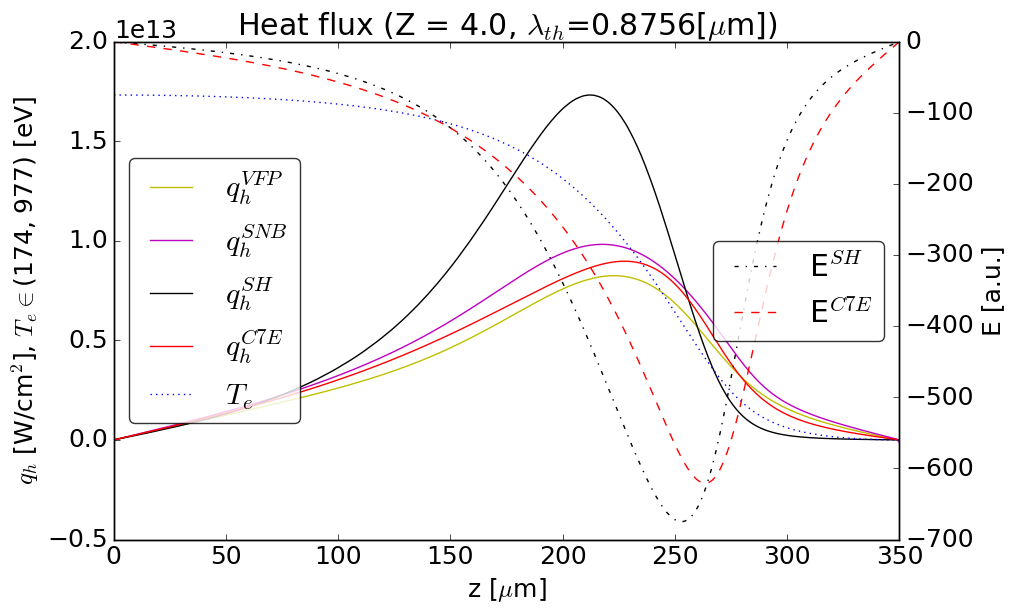
\includegraphics[width=1.0\textwidth]{../VFPdata/C7_heatflux_12ps.png} \\ 
      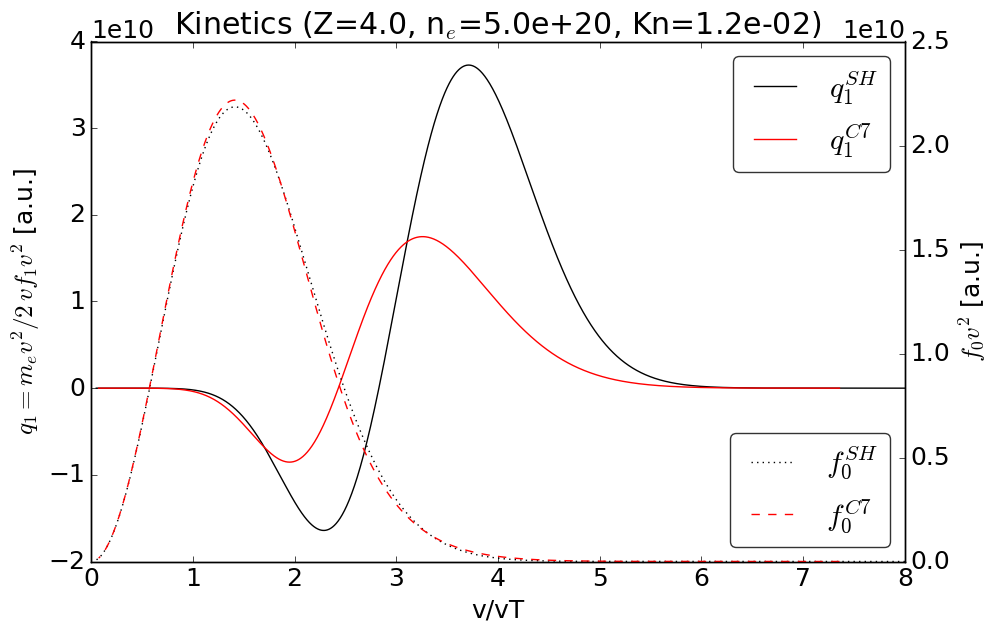
\includegraphics[width=1.0\textwidth]{../VFPdata/C7_kinetics_12ps.png}
    \end{tabular}
  \caption{
  Philippe's preferred test $\Zbar = 4$ at 12 ps.  
  }
  \end{center}
  \label{fig:Philippe_VFP_12ps}
\end{figure}

\begin{figure}[tbh]
  \begin{center}
    \begin{tabular}{c}
      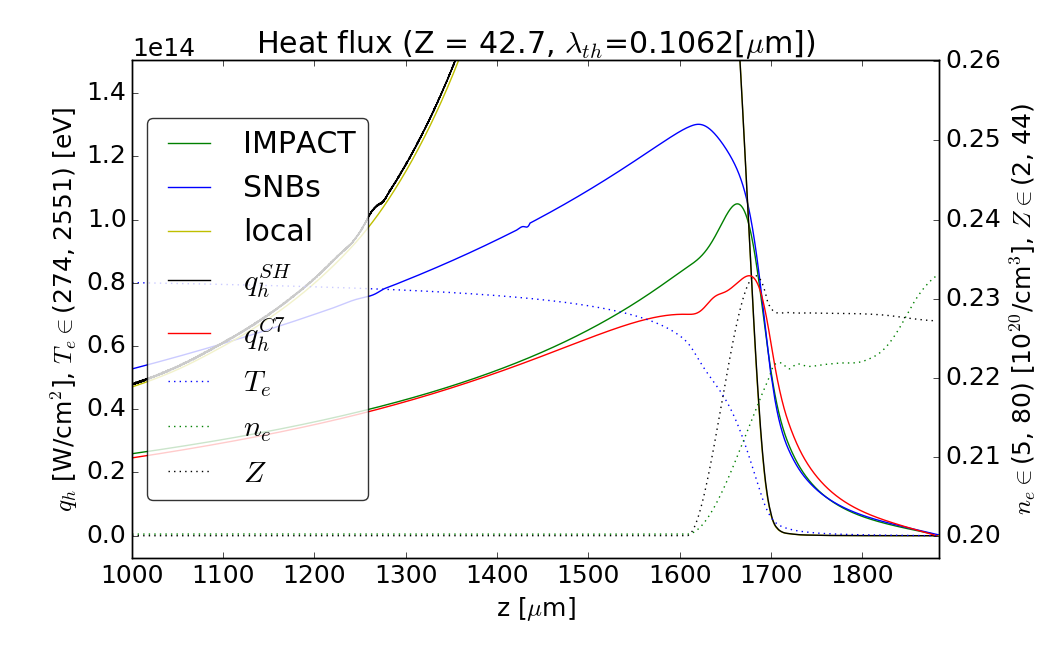
\includegraphics[width=1.0\textwidth]{../VFPdata/GD_Hohlraum/fluxes_10ps.png} \\
      %\includegraphics[width=1.0\textwidth]{../VFPdata/GD_Hohlraum/diffusion_fluxes_10ps.png} 
      %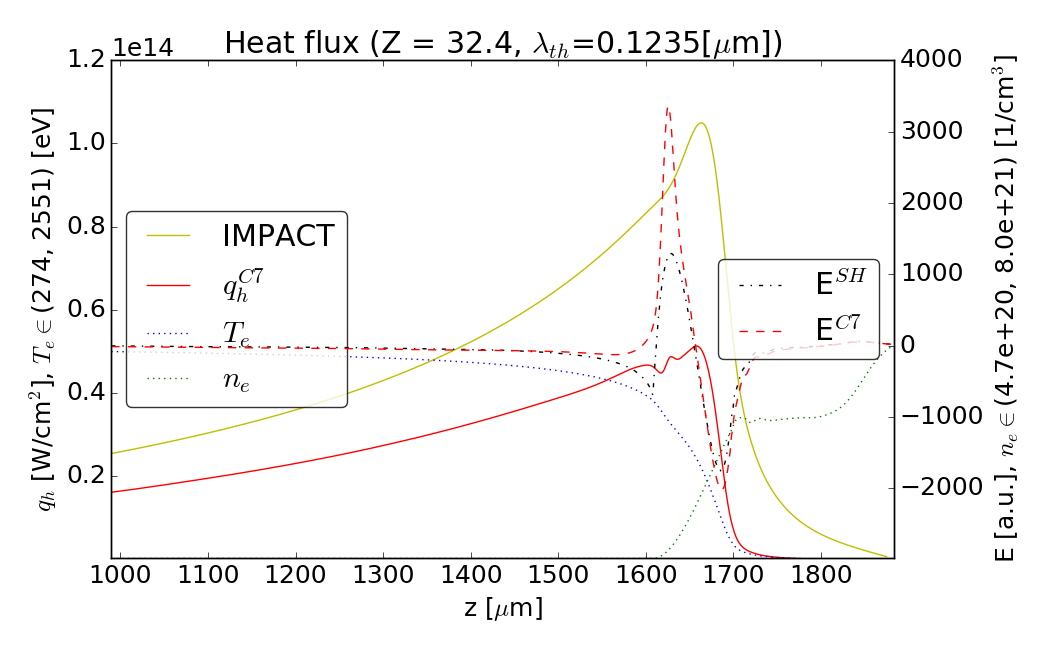
\includegraphics[width=1.0\textwidth]{../VFPdata/GD_Hohlraum/fluxes_Efield_10ps.png} \\ 
      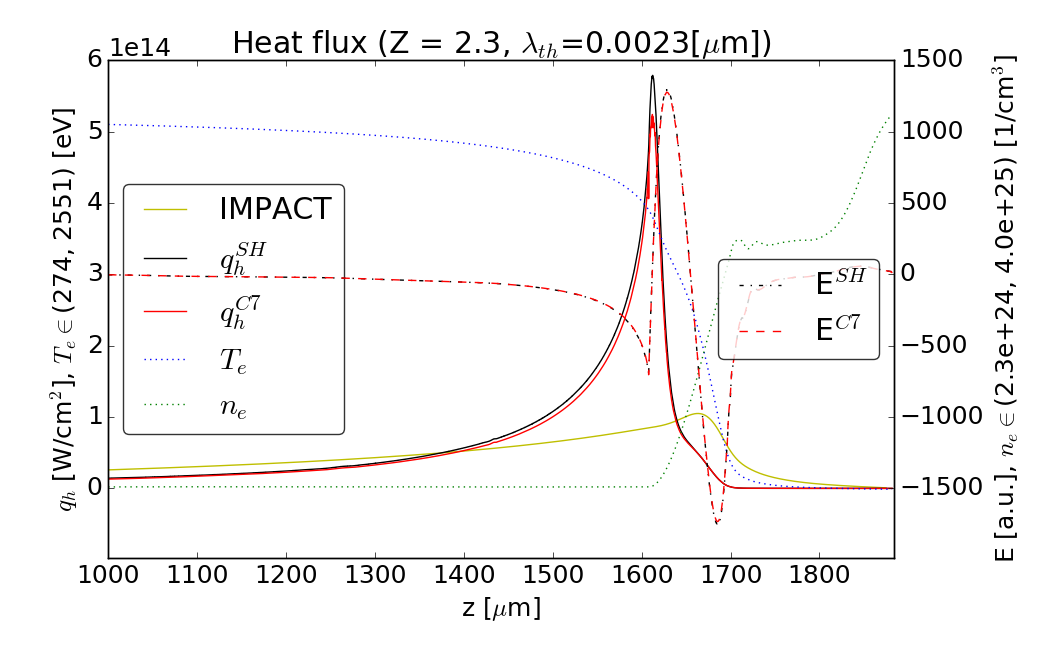
\includegraphics[width=1.0\textwidth]{../VFPdata/GD_Hohlraum/diffusion_fluxes_Efield_10ps.png} 
    \end{tabular}
  \caption{
  }
  \end{center}
  \label{fig:Gd_VFP_10ps_heatflux}
\end{figure}

\begin{figure}[tbh]
  \begin{center}
    \begin{tabular}{c}
       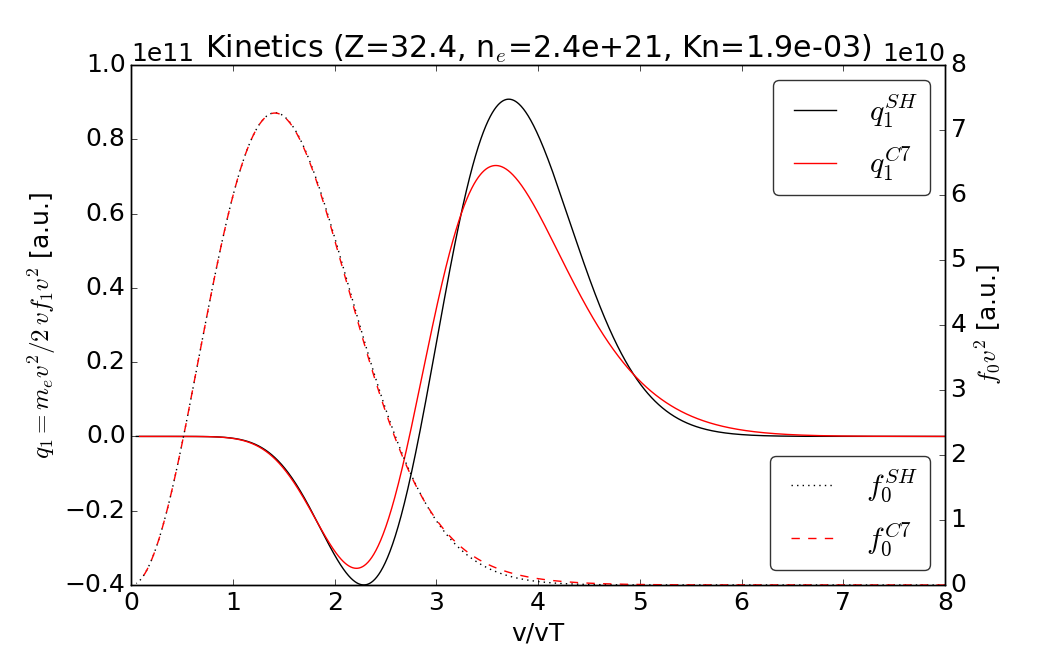
\includegraphics[width=1.0\textwidth]{../VFPdata/GD_Hohlraum/kinetics_10ps_xpointmax.png} \\ 
      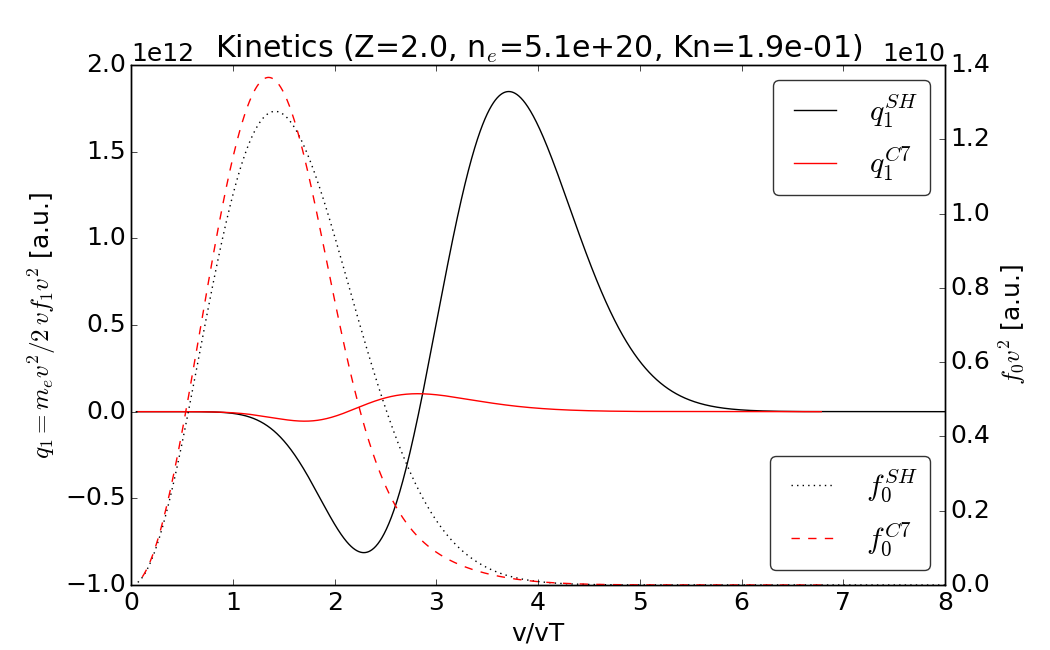
\includegraphics[width=1.0\textwidth]{../VFPdata/GD_Hohlraum/kinetics_10ps_xpoint_1605microns.png}
    \end{tabular}
  \caption{
  Kinetics profiles for max(flux) point and 1605 microns point for the case of 10ps VFP temperature profile, ne and Z Hydra profiles. 
  }
  \end{center}
  \label{fig:Gd_VFP_10ps_kinetics}
\end{figure}

\begin{figure}[tbh]
  \begin{center}
    \begin{tabular}{c}
      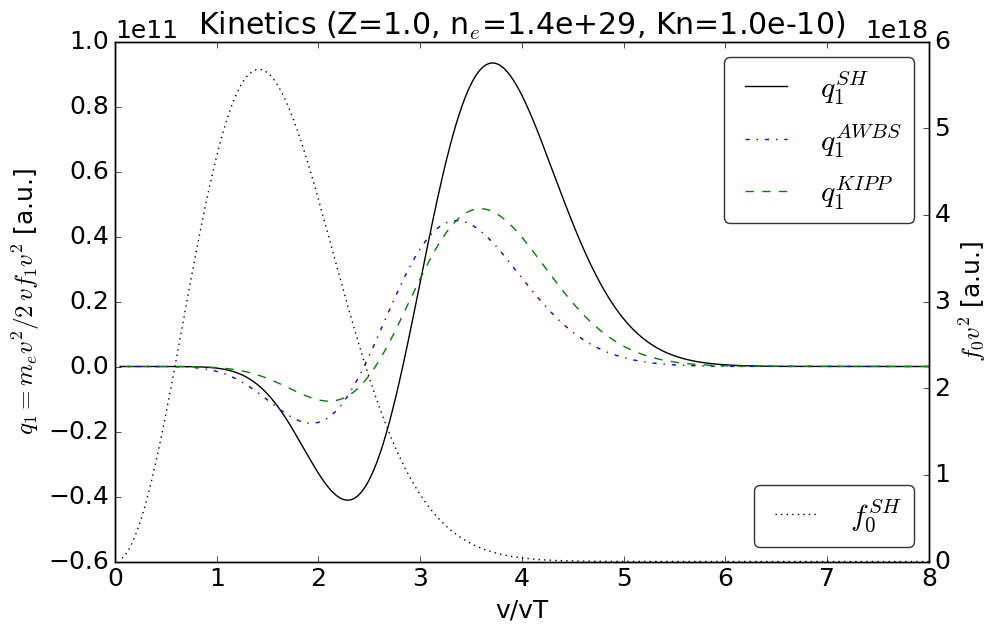
\includegraphics[width=1.0\textwidth]{../VFPdata/KIPP_q_kinetics.png} \\
      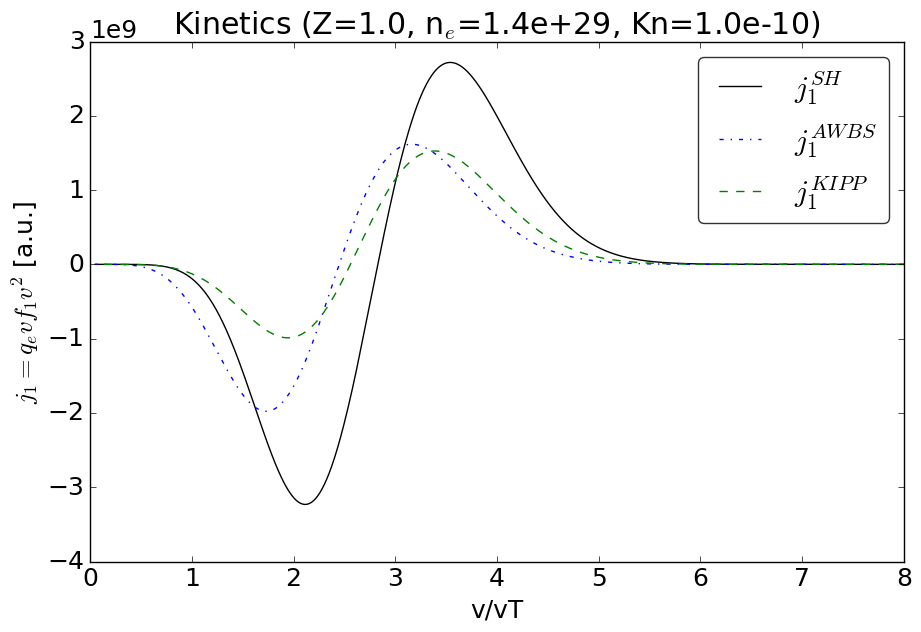
\includegraphics[width=1.0\textwidth]{../VFPdata/KIPP_j_kinetics.png}
    \end{tabular}
  \caption{KIPP (by Johnathan) vs AWBS using 
  $\mfpei^* = \frac{\Zbar + 0.24}{\Zbar + 4.2}\mfpei, \Zbar=1, 
  \vth = \sqrt{\frac{\kB T_e}{\me}}$ 
  $f_1^{SH} = -\mfpei^*(v) \left(\frac{v^2}{2 \vth^2} - 4\right) 
  \frac{\vn\cdot\nabla T_e}{T_e} \fM,\quad 
  f_1^{KIPP} = -\mfpei^*(v) \left(\frac{3}{16}\frac{v^2}{\vth^2} - 1 
  - \frac{3}{2}\frac{\vth^2}{v^2} \right) 
  \frac{\vn\cdot\nabla T_e}{T_e} \fM$.
  }
  \end{center}
  \label{fig:}
\end{figure}

\begin{figure}[tbh]
  \begin{center}
    \begin{tabular}{c}
      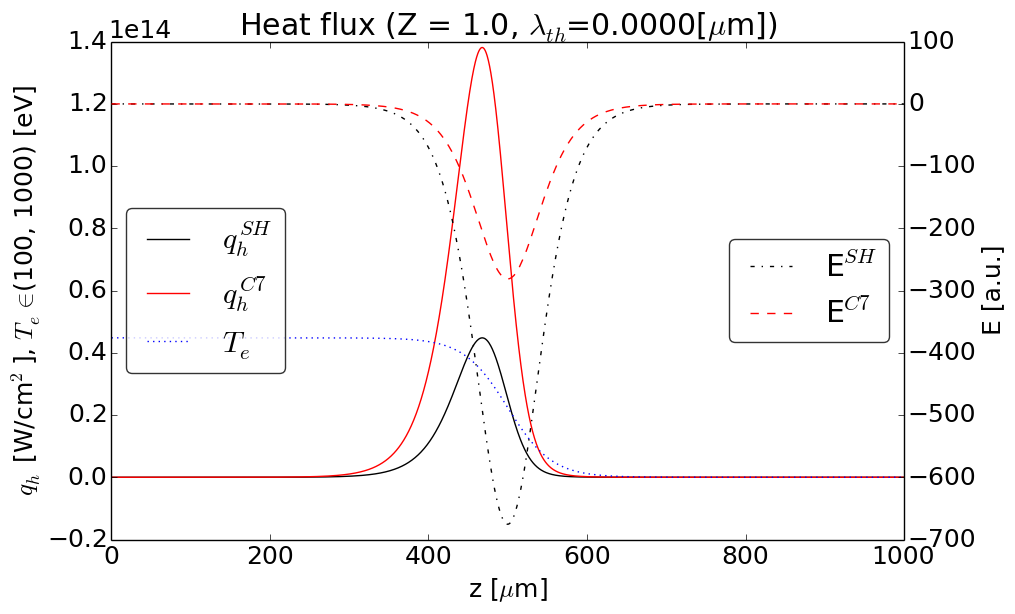
\includegraphics[width=1.0\textwidth]{../results/fe_analysis/figs/P5_diffusive_heatflux_Z1_decelerating_Ezerothiter.png} \\
      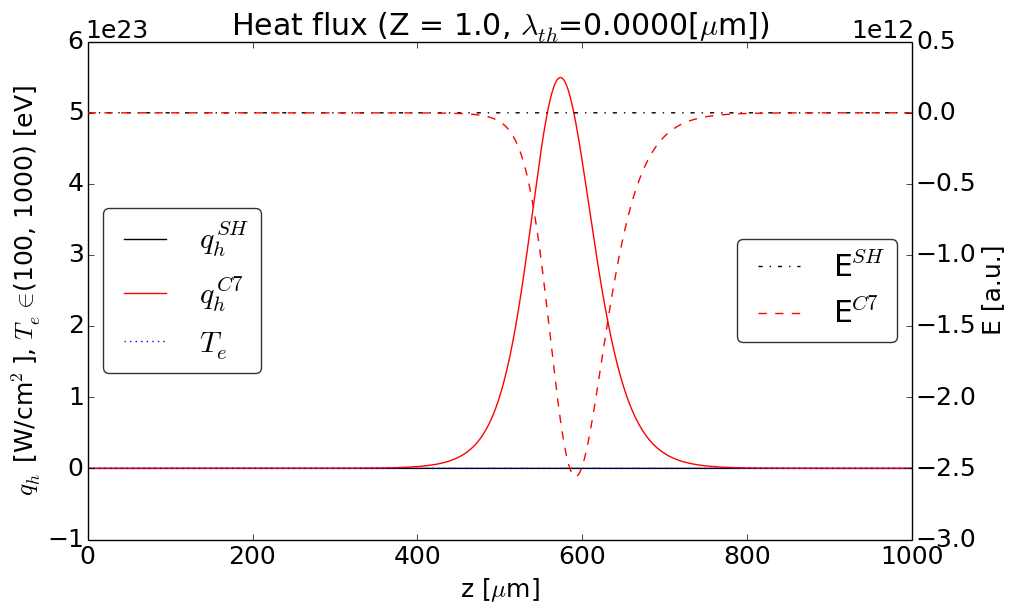
\includegraphics[width=1.0\textwidth]{../results/fe_analysis/figs/P5_diffusive_heatflux_Z1_accelerating_Ezerothiter.png}
    \end{tabular}
  \caption{
  Decelerating (top) vs. accelerating (bottom) computations. 
  Zeroth E field iteration, i.e.
  no E field effect, of the diffusion regime conditions.
  }
  \end{center}
  \label{fig:}
\end{figure}

\clearpage

%\begin{figure}[tbh]
%  \begin{center}
%    \begin{tabular}{c}
%      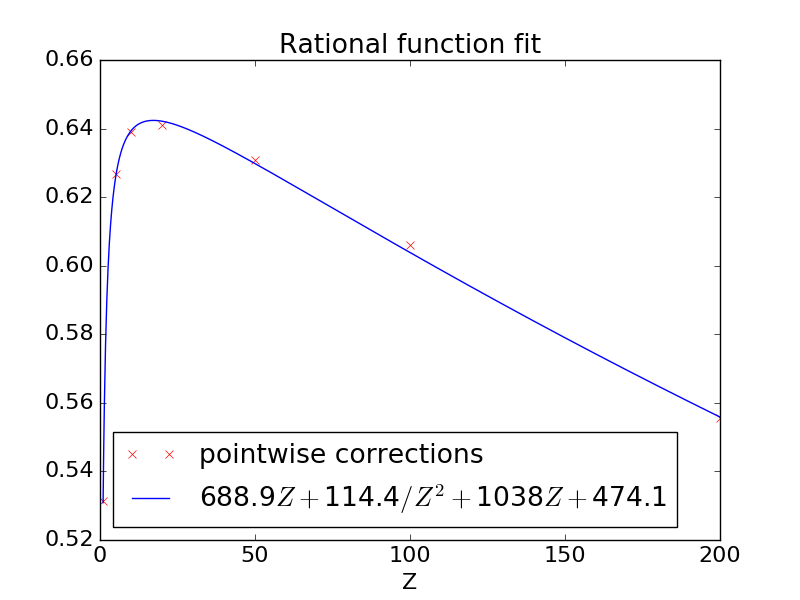
\includegraphics[width=0.55\textwidth]{../results/fe_analysis/figs/AWBScorrection_fit.png} 
%    \end{tabular}
%  \caption{
%  Analytic fit to the~Z correction 
%  ($\nue^* = \frac{688.9 \Zbar + 114.4}{\Zbar^2 + 
%  1038 \Zbar + 474.1} \nue$, where $\nue = \nuei / \Zbar$) 
%  of the~diffusion asymptotic of AWBS with respect to SH.
%  }
%  \end{center}
%  \label{fig:}
%\end{figure}

%% The Appendices part is started with the command \appendix;
%% appendix sections are then done as normal sections
%% \appendix

%% \section{}
%% \label{}

%% References
%%
%% Following citation commands can be used in the body text:
%% Usage of \cite is as follows:
%%   \cite{key}         ==>>  [#]
%%   \cite[chap. 2]{key} ==>> [#, chap. 2]
%%

%% References with bibTeX database:

\bibliographystyle{elsarticle-num}
\bibliography{NTH}

%% Authors are advised to submit their bibtex database files. They are
%% requested to list a bibtex style file in the manuscript if they do
%% not want to use elsarticle-num.bst.

%% References without bibTeX database:

% \begin{thebibliography}{00}

%% \bibitem must have the following form:
%%   \bibitem{key}...
%%

% \bibitem{}

% \end{thebibliography}


\end{document}

%%
%% End of file 
